%% ===================================================================
%% Báo cáo môn IT701100 -- Mô hình đồ thị có xác suất (HK1 2026--2027)
%% Dựa trên thực nghiệm 07: notebooks/07_coupon_rules_original_habits.ipynb
%% Template: Springer Nature LaTeX Template, Version 3.1 (December 2024)
%%
%% BIÊN DỊCH BẰNG XeLaTeX (vì tiếng Việt có dấu):
%%     latexmk -xelatex report.tex
%% hoặc: xelatex report && bibtex report && xelatex report && xelatex report
%% Trên Overleaf: Menu -> Compiler -> XeLaTeX.
%% ===================================================================
\documentclass[pdflatex,sn-mathphys-num]{sn-jnl}% Math and Physical Sciences Numbered Reference Style

%%%% Standard Packages
\usepackage{fontspec}% font Unicode cho XeLaTeX; mặc định Latin Modern, có đủ dấu tiếng Việt
\usepackage{graphicx}%
\usepackage{multirow}%
\usepackage{amsmath,amssymb,amsfonts}%
\usepackage{amsthm}%
\usepackage{mathrsfs}%
\usepackage[title]{appendix}%
\usepackage{xcolor}%
\usepackage{textcomp}%
\usepackage{manyfoot}%
\usepackage{booktabs}%
\usepackage{array}%
%%%%

%% ----- Việt hoá các nhãn mà class sn-jnl in sẵn bằng tiếng Anh -----
\renewcommand{\figurename}{Hình}
\renewcommand{\tablename}{Bảng}
\renewcommand{\refname}{Tài liệu tham khảo}
\renewcommand{\abstractname}{Tóm tắt}
\renewcommand{\appendixname}{Phụ lục}
\renewcommand{\keywordname}{Từ khóa}
%% Chữ nối giữa hai tác giả: "và" thay cho "and"
\makeatletter
\def\au@and{\ifnum\punctcount=2\ và\else\unskip, \advance\punctcount by -1 \fi}%
\makeatother
%% Tiếng Việt không ngắt từ giữa âm tiết: tắt hyphenation, cho phép giãn dòng thêm một chút
\hyphenpenalty=10000 \exhyphenpenalty=10000 \emergencystretch=2em

%% ----- Lệnh viết tắt dùng trong bài -----
\newcommand{\var}[1]{\texttt{#1}}                 % tên biến của dữ liệu
\newcommand{\doop}{\mathrm{do}}                   % toán tử do(.)
\newcommand{\PaY}{\mathrm{Pa}(Y)}                 % parents của Y
\newcommand{\ATE}{\mathrm{ATE}}
\newcolumntype{L}[1]{>{\raggedright\arraybackslash}p{#1}}

\raggedbottom

\begin{document}

\title[CBN trên dữ liệu UCI In-Vehicle Coupon]{Causal Bayesian Network trên dữ liệu UCI In-Vehicle Coupon: mô hình cơ sở B0 và hai mở rộng neural network H1, H2}

%% TODO (nhóm): bổ sung tên trường/khoa vào \affil và e-mail nếu cần.
\author[1]{\fnm{Lê Anh} \sur{Tuấn}}
\author[1]{\fnm{Tô Hoàng} \sur{Đạo}}

\affil[1]{Học viên cao học, môn IT701100 Mô hình đồ thị có xác suất, HK1 2026--2027. Mã số học viên: 252805005 (Lê Anh Tuấn), 252805401 (Tô Hoàng Đạo)}

\abstract{Báo cáo ước lượng hiệu ứng nhân quả của \emph{hạn dùng coupon} (2 giờ so với 1 ngày) lên xác suất tài xế chấp nhận coupon, trên bộ dữ liệu UCI In-Vehicle Coupon Recommendation (sau khi lọc còn 12.197 dòng tình huống của 587 người trả lời). Mô hình cơ sở B0 là một Causal Bayesian Network rời rạc 18 nút: DAG học bằng Hill Climbing dưới một bộ luật miền cấm 212 trên 306 mũi tên, CPD ước lượng bằng BDeu. Mỗi mở rộng chỉ đổi một thành phần của B0: H1 thay CPD của outcome bằng một MLP trên đúng DAG của B0; H2 học DAG bằng NOTEARS-MLP với cùng bộ luật rồi ước lượng CPD như B0. Qua năm lần chạy theo cặp (chia dữ liệu theo người, 70/15/15), ba mô hình dự đoán gần ngang nhau (AUROC 0,726 / 0,731 / 0,733; log loss 0,608 / 0,598 / 0,617) và cho cùng một kết luận can thiệp: ATE chuẩn hoá trên TEST là $-$0,157 (B0), $-$0,155 (H1) và $-$0,148 (H2), tức tỉ lệ chấp nhận giảm từ khoảng 64\% xuống khoảng 49\% khi đổi hạn từ 1 ngày sang 2 giờ. Cả 15 khoảng tin cậy bootstrap 95\% nằm dưới 0, và hai refuter của DoWhy đạt trên cả 10 DAG. Con số này chỉ mang nghĩa nhân quả khi không có confounder bị bỏ sót, và outcome là ý định khai báo trong tình huống giả định chứ không phải hành vi thật. H2 cho ATE gần 0 hơn B0 ở cả năm lần chạy, nhiều khả năng vì 14,3\% dòng TEST của nó rơi vào ô CPD không có dữ liệu TRAIN.}

\keywords{Causal Bayesian Network, học cấu trúc, NOTEARS, neural CPD, do-calculus, DoWhy, In-Vehicle Coupon}

\maketitle

%% ===================================================================
\section{Giới thiệu}\label{sec:intro}
%% (mục 2.1 của rubric)

Một doanh nghiệp phát coupon cho tài xế qua màn hình xe phải chọn hạn dùng cho coupon: ngắn (2 giờ) hay dài (1 ngày). Đây là biến mà doanh nghiệp tự đặt được với chi phí gần như bằng 0, nên câu hỏi tự nhiên là một câu hỏi can thiệp chứ không phải câu hỏi dự đoán:

\begin{quote}
\emph{Nếu mọi coupon đều được đặt hạn dùng 2 giờ thay vì 1 ngày, tỉ lệ tài xế chấp nhận coupon thay đổi bao nhiêu?}
\end{quote}

Báo cáo trả lời câu hỏi này trên bộ dữ liệu UCI In-Vehicle Coupon Recommendation \cite{uci603,wang2017}. So sánh thô hai nhóm coupon là chưa đủ, vì hai nhóm khác nhau từ đầu: loại quán và hoàn cảnh lái xe vừa quyết định coupon được gán hạn nào, vừa quyết định người ta có thích coupon đó không. Trên TRAIN của lần chia đầu tiên, tỉ lệ coupon hạn 2 giờ đi từ 30\% (quán bar) đến 56\% (quán cà phê), còn tỉ lệ chấp nhận coupon hạn 1 ngày đi từ 42\% đến 82\% giữa các loại quán (Hình~\ref{fig:confounding}).

Causal Bayesian Network (CBN) \cite{pearl2009,koller2009} là khung phù hợp để làm mốc so sánh vì ba lý do. Thứ nhất, nó tách bạch ba việc: sơ đồ nhân quả (DAG), điều kiện để hiệu ứng tính được từ dữ liệu quan sát (nhận diện), và việc ước lượng các xác suất có điều kiện (CPD). Thứ hai, khi mọi biến đều rời rạc thì mỗi CPD là một bảng đếm đọc được bằng mắt, và truy vấn $\doop(\cdot)$ được tính chính xác bằng tra bảng. Thứ ba, vì các thành phần tách rời, có thể thay \emph{đúng một} thành phần bằng một phương pháp deep learning và quy mọi khác biệt về kết quả cho thay đổi đó.

Theo đề bài, báo cáo so sánh ba mô hình trên cùng dữ liệu, cùng cách chia và cùng nhóm tham chiếu TEST:
\begin{itemize}
\item \textbf{B0} (mốc so sánh): DAG học bằng Hill Climbing của \texttt{pgmpy} \cite{pgmpy2024} dưới ràng buộc miền; CPD đếm trong dữ liệu, làm trơn bằng BDeu \cite{heckerman1995}.
\item \textbf{H1}: giữ nguyên DAG của B0, thay CPD của $Y$ bằng một MLP nhỏ. Thay đổi duy nhất là \emph{cách tính xác suất của $Y$}.
\item \textbf{H2}: học DAG bằng NOTEARS-MLP \cite{zheng2018,zheng2020} với cùng ràng buộc, CPD ước lượng như B0. Thay đổi duy nhất là \emph{cách tìm DAG}.
\end{itemize}

Kết quả chính: ba mô hình cho cùng câu trả lời. Đặt hạn 2 giờ thay cho 1 ngày đi kèm xác suất chấp nhận thấp hơn khoảng 15--16 điểm phần trăm (từ khoảng 64\% xuống khoảng 49\%), ổn định qua năm cách chia dữ liệu; thay thành phần truyền thống bằng neural network không làm đổi kết luận can thiệp và chỉ cải thiện dự đoán ở mức rất nhỏ.

\textbf{Bố cục.} Mục~\ref{sec:related} điểm lại các công trình liên quan; Mục~\ref{sec:problem} phát biểu bài toán; Mục~\ref{sec:methods} mô tả ba mô hình và giao thức chung; Mục~\ref{sec:design} trình bày thiết kế thực nghiệm; Mục~\ref{sec:results} báo cáo Bảng A, B, C; Mục~\ref{sec:conclusion} kết luận và nêu hạn chế; Mục~\ref{sec:qa} trả lời các câu hỏi bảo vệ. Các mục này ứng với mục 2.1--2.7 và 2.9 của đề bài; mục 2.8 là phần Tóm tắt.

%% ===================================================================
\section{Công trình liên quan}\label{sec:related}
%% (mục 2.2 của rubric)

\textbf{CBN và can thiệp.} Bayesian Network gồm một DAG và một CPD cho mỗi nút \cite{koller2009}. Khi các mũi tên được đọc theo nghĩa nhân quả, can thiệp $\doop(T{=}t)$ ứng với việc xoá mọi mũi tên đi vào $T$ rồi đặt $T=t$ (truncated factorization), và tiêu chí backdoor cho biết tập biến nào cần giữ cố định để hiệu ứng tính được từ dữ liệu quan sát \cite{pearl2009}. Chuẩn hoá theo một quần thể tham chiếu (standardization, g-formula) là cách ước lượng tương ứng \cite{hernan2020}.

\textbf{Học cấu trúc truyền thống.} Các phương pháp dựa trên điểm tìm DAG tối ưu một hàm điểm bằng tìm kiếm tham lam, tiêu biểu là Hill Climbing với các điểm K2 \cite{cooper1992}, BDeu \cite{heckerman1995} hay BIC, và GES \cite{chickering2002}. Các phương pháp dựa trên kiểm định như PC \cite{spirtes2000} xoá cạnh giữa hai biến độc lập có điều kiện; MMHC \cite{tsamardinos2006} lai hai hướng. \texttt{pgmpy} \cite{pgmpy2024} và \texttt{bnlearn} \cite{scutari2010} cài đặt các thuật toán này và cho phép đưa tri thức miền vào dưới dạng cạnh cấm, cạnh bắt buộc. Dữ liệu quan sát chỉ xác định DAG đến lớp tương đương Markov, nên chiều của nhiều cạnh phải do tri thức miền quyết định.

\textbf{Học cấu trúc bằng tối ưu liên tục.} NOTEARS \cite{zheng2018} đổi bài toán tổ hợp thành bài toán tối ưu liên tục nhờ một hàm $h(A)$ bằng 0 đúng khi đồ thị có trọng số $A$ không có chu trình. NOTEARS-MLP \cite{zheng2020} mở rộng sang quan hệ phi tuyến bằng cách cho mỗi nút một MLP và đọc độ mạnh cạnh từ trọng số lớp đầu. DAG-GNN \cite{yu2019} dùng autoencoder biến phân trên đồ thị; GOLEM \cite{ng2020} và DAGMA \cite{bello2022} đề xuất hàm mục tiêu và ràng buộc phi chu trình khác. Reisach và cộng sự \cite{reisach2021} chỉ ra rằng kết quả tốt của nhóm phương pháp này trên dữ liệu mô phỏng có thể đến từ thang đo của biến chứ không từ cấu trúc nhân quả. Các khảo sát \cite{vowels2022} cũng lưu ý rằng trọng số cạnh là đại lượng nội bộ của thuật toán, không phải hiệu ứng nhân quả. Báo cáo này chọn NOTEARS-MLP cho H2 vì nó nhận ràng buộc miền một cách tự nhiên qua mask trên ma trận kề; các phương pháp còn lại chỉ được nhắc ở đây.

\textbf{Neural network làm CPD.} CPD dạng bảng có số ô tăng theo cấp số nhân với số parents; Koller và Friedman \cite{koller2009} trình bày các CPD có cấu trúc (cây, noisy-or, mô hình logistic) để chia sẻ tham số giữa các ô. Dùng một MLP làm CPD là bước tiếp theo của ý tưởng đó: mạng học một hàm chung cho mọi tổ hợp giá trị của parents. Thư viện DoWhy \cite{dowhy2020} cũng cho phép gán một bộ phân loại bất kỳ làm cơ chế nhân quả của một nút.

\textbf{Dữ liệu.} Bộ In-Vehicle Coupon Recommendation được Wang và cộng sự \cite{wang2017} thu qua một khảo sát trên Amazon Mechanical Turk và dùng để đánh giá mô hình phân loại diễn giải được. Theo hiểu biết của nhóm, bộ dữ liệu này chủ yếu được dùng cho bài toán dự đoán; báo cáo này dùng nó cho một câu hỏi can thiệp.

%% ===================================================================
\section{Phát biểu bài toán}\label{sec:problem}
%% (mục 2.3 của rubric)

\subsection{Quần thể và đơn vị phân tích}

Dữ liệu là một khảo sát trong đó người tham gia xem các \emph{tình huống lái xe giả định} (đang đi đâu, mấy giờ, thời tiết thế nào, chở ai), rồi một coupon hiện trên màn hình xe (loại quán, hạn dùng) và họ trả lời có dùng coupon đó không \cite{wang2017}. Mỗi dòng là \emph{một lần hỏi}; trong file gốc mỗi người trả lời từ 6 đến 34 dòng (phổ biến nhất là 22 dòng). Quần thể mục tiêu là phân phối các \emph{dòng tình huống đủ điều kiện} (Mục~\ref{sec:data}), chuẩn hoá trên tập TEST; nó không mặc nhiên đại diện cho mọi tài xế hay mọi coupon.

\subsection{Biến và thứ tự thời gian}

Mô hình dùng 18 biến rời rạc, xếp thành bốn tầng theo thời gian (Bảng~\ref{tab:vars}): đặc điểm của người trả lời có trước cuộc khảo sát; kịch bản lái xe và loại coupon được bảng hỏi đưa ra; hạn coupon $T$ được gán cùng kịch bản; câu trả lời $Y$ đến sau cùng.

\begin{itemize}
\item \textbf{Treatment} $T$ = hạn coupon: $T=0$ là hạn 1 ngày (nhóm control), $T=1$ là hạn 2 giờ (nhóm treatment).
\item \textbf{Outcome} $Y \in \{0,1\}$: 1 nếu người trả lời nói sẽ chấp nhận coupon.
\item \textbf{Biến nền} $C$: 16 biến còn lại, đều được đo trước $T$.
\end{itemize}

\begin{table}[t]
\caption{Từ điển biến: 18 nút của DAG sau tiền xử lý (12.197 dòng). Tầng 1 và 2 đều có trước $T$.}\label{tab:vars}
\begin{tabular}{@{}L{3.3cm}L{3.7cm}L{4.7cm}@{}}
\toprule
Biến & Ý nghĩa & Các mức \\
\midrule
\multicolumn{3}{@{}l}{\emph{Tầng 1 -- người trả lời (có thể $\to Y$; cấm $\to T$)}} \\
\var{Bar}, \var{CoffeeHouse}, \var{CarryAway}, \var{RestaurantLessThan20}, \var{Restaurant20To50} & Thói quen: số lần mỗi tháng đến từng loại quán & \var{low} (never, less1), \var{mid} (1\textasciitilde 3), \var{high} (4\textasciitilde 8, gt8), \var{missing} \\
\var{age\_bin} & Nhóm tuổi & <26, 26--35, 36--50, 50+ \\
\var{income\_bin} & Nhóm thu nhập (USD/năm) & <37,5k; 37,5--75k; 75k+ \\
\var{gender} & Giới tính & Female, Male \\
\var{has\_children} & Có con & 0, 1 \\
\addlinespace[2pt]
\multicolumn{3}{@{}l}{\emph{Tầng 2 -- kịch bản (có thể $\to T$ và $\to Y$)}} \\
\var{coupon} & Loại quán của coupon & Coffee House, Restaurant(<20), Carry out \& Take away, Bar, Restaurant(20--50) \\
\var{destination} & Điểm đến của chuyến đi & No Urgent Place, Home, Work \\
\var{time\_bin} & Giờ trong ngày & morning (7AM, 10AM), afternoon (2PM), evening (6PM, 10PM) \\
\var{passenger} & Người đi cùng & Alone, Friend(s), Partner, Kid(s) \\
\var{weather} & Thời tiết & Sunny, Snowy, Rainy \\
\var{dist} & Thời gian lái xe tới quán (phút) & <15, 15--25, 25+ \\
\var{direction\_same} & Quán cùng hướng với điểm đến & 0, 1 \\
\addlinespace[2pt]
\multicolumn{3}{@{}l}{\emph{Tầng 3 -- treatment và tầng 4 -- outcome}} \\
\var{T} & Hạn coupon & 0 = 1 ngày (6.604 dòng), 1 = 2 giờ (5.593 dòng) \\
\var{Y} & Chấp nhận coupon & 1 = có (7.032 dòng), 0 = không (5.165 dòng) \\
\botrule
\end{tabular}
\end{table}

\subsection{Estimand}

Đại lượng cần ước lượng là hiệu ứng trung bình của việc đổi hạn (average treatment effect):
\begin{equation}\label{eq:ate}
\ATE = P\big(Y{=}1 \mid \doop(T{=}1)\big) - P\big(Y{=}1 \mid \doop(T{=}0)\big),
\end{equation}
tức tỉ lệ chấp nhận nếu \emph{ép} mọi coupon có hạn 2 giờ trừ tỉ lệ chấp nhận nếu ép mọi coupon có hạn 1 ngày, giữ nguyên mọi biến nền của nhóm tham chiếu.

\subsection{DAG và giả định}

DAG không được vẽ tay toàn bộ mà được \emph{học} từ dữ liệu trong khuôn khổ một bộ luật miền (Mục~\ref{sec:rules}). Phần cấu trúc mà câu hỏi cần gồm ba loại mũi tên: kịch bản $\to T$ (cái gì quyết định hạn coupon), biến nền $\to Y$ (cái gì quyết định việc chấp nhận) và $T \to Y$. Biến trỏ vào cả $T$ lẫn $Y$ là confounder, ví dụ loại quán tạo ra backdoor path $T \leftarrow \var{coupon} \to Y$. Kết quả chỉ đọc được theo nghĩa nhân quả dưới các giả định sau:

\begin{itemize}
\item[G1] Cơ chế gán hạn dựa trên kịch bản, không trực tiếp dựa trên hồ sơ cá nhân của người trả lời.
\item[G2] Tập biến điều chỉnh chặn đủ mọi nguyên nhân chung của $T$ và $Y$ (không có confounder bị bỏ sót).
\item[G3] Can thiệp chỉ đổi hạn coupon, không đổi gì khác (consistency).
\item[G4] Trong các hoàn cảnh đem so sánh phải có cả hai loại hạn (overlap); ô thiếu một loại hạn đòi hỏi ngoại suy.
\item[G5] $Y$ là ý định khai báo trong khảo sát, không phải hành vi sử dụng thực tế.
\item[G6] Các khối dòng liên tiếp có cùng hồ sơ cá nhân được coi là của cùng một người.
\end{itemize}

G1 và G4 kiểm được một phần bằng dữ liệu (Mục~\ref{sec:overlap}); G2, G3, G5 là giả định, không kiểm chứng được từ bộ dữ liệu này.

\subsection{Ba bài toán con}

Báo cáo tách ba việc thường bị gộp làm một:
\begin{itemize}
\item \textbf{Causal discovery} (tìm DAG): B0 dùng Hill Climbing, H2 dùng NOTEARS-MLP, cùng trên TRAIN và cùng bộ luật. Dữ liệu chỉ xác định cấu trúc đến lớp tương đương; chiều của cạnh giữa các nhóm biến do bộ luật quyết định, còn chiều của cạnh trong cùng một nhóm (ví dụ giữa hai thói quen) không phải là kết luận nhân quả.
\item \textbf{Nhận diện} (identification): chỉ dựa vào hình dạng của DAG, trả lời liệu $P(Y \mid \doop(T))$ có viết được theo phân phối quan sát hay không và phải điều chỉnh theo biến nào. Bước này được chạy lại bằng DoWhy cho từng DAG.
\item \textbf{Ước lượng} (estimation): bài toán thống kê, ước lượng $P(Y \mid T, Z)$ bằng bảng đếm (B0, H2) hoặc bằng MLP (H1) rồi chuẩn hoá trên TEST.
\end{itemize}

Mỗi mở rộng cần thêm giả định riêng. H1 dùng lại DAG và công thức nhận diện của B0; nó giả định thêm rằng hàm trơn do MLP học được ngoại suy hợp lý sang các tổ hợp parents ít hoặc không có dữ liệu, điều không kiểm được ở chính các ô trống đó. H2 giả định rằng tối ưu liên tục với phạt thưa và ràng buộc phi chu trình cho ra một đồ thị tương thích với cùng tri thức miền; vì DAG thay đổi nên phải nhận diện lại, và trọng số cạnh không được đọc như hiệu ứng nhân quả.

%% ===================================================================
\section{Phương pháp}\label{sec:methods}
%% (mục 2.4 của rubric)

Ba mô hình dùng chung tập biến, trạng thái của biến, bộ luật DAG, cách chia dữ liệu, giao thức dự đoán và giao thức can thiệp. Bảng~\ref{tab:models} tóm tắt điểm khác nhau có kiểm soát giữa chúng; mọi siêu tham số nằm trong một đối tượng cấu hình duy nhất (Bảng~\ref{tab:config}).

\begin{table}[t]
\caption{Ba mô hình và thay đổi duy nhất của mỗi mở rộng so với B0.}\label{tab:models}
\begin{tabular}{@{}lL{3.6cm}L{3.9cm}L{3.3cm}@{}}
\toprule
 & Cách tìm DAG & CPD của $Y$ & Khác B0 ở \\
\midrule
B0 & Hill Climbing (\texttt{pgmpy}), có ràng buộc & Bảng đếm, làm trơn BDeu & (mốc so sánh) \\
H1 & DAG của B0 (cùng seed) & MLP, liệt kê lại thành bảng & cách tính xác suất của $Y$ \\
H2 & NOTEARS-MLP có mask, cùng ràng buộc & Bảng đếm, làm trơn BDeu & cách tìm DAG \\
\botrule
\end{tabular}
\footnotetext{CPD của 17 nút còn lại luôn là bảng đếm làm trơn BDeu với cùng equivalent sample size.}
\end{table}

\subsection{Ràng buộc DAG dùng chung}\label{sec:rules}

Trước khi học, mỗi nút được gán một danh sách \emph{parents được phép} kèm lý do (Bảng~\ref{tab:rules}); mọi mũi tên khác đều bị cấm. Có hai loại lý do: \emph{nút gốc} (không biến nào trong bài làm đổi được thời tiết, tuổi hay giới tính) và \emph{thứ tự thời gian} (cái có sau không gây ra cái có trước). Trong 306 mũi tên có thể vẽ giữa 18 nút, 212 bị cấm và 94 được phép. Hai điểm đáng chú ý: (i) năm thói quen là đặc điểm có trước cuộc khảo sát nên không nhận mũi tên nào từ kịch bản hay từ coupon; (ii) cạnh duy nhất được phép đi từ nhóm người trả lời sang nhóm kịch bản là $\var{has\_children} \to \var{passenger}$, vì hành khách là trẻ em gần như chỉ xuất hiện ở người có con (Mục~\ref{sec:overlap}).

Từ bộ luật sinh ra ba thứ: danh sách cạnh cấm và cạnh bắt buộc cho \texttt{pgmpy} (B0), ma trận mask $M \in \{0,1\}^{18\times18}$ với $M_{ij}=1$ khi mũi tên $i \to j$ được phép (H2), và hàm \texttt{check\_dag} kiểm tự động mọi DAG do thuật toán sinh ra, trả về danh sách vi phạm kèm số của luật. Mọi DAG phải qua \texttt{check\_dag} trước khi được dùng.

\begin{table}[t]
\caption{Bộ luật DAG: parents được phép của từng nút. Mọi mũi tên không nằm trong cột thứ ba đều bị cấm.}\label{tab:rules}
\setlength{\tabcolsep}{4pt}
\begin{tabular}{@{}cL{2.5cm}L{3.3cm}cL{4.4cm}@{}}
\toprule
Luật & Áp cho nút & Parents được phép & Cấm & Lý do \\
\midrule
1 & \var{weather}, \var{age\_bin}, \var{gender} & (không có) & 51 & Nút gốc: không biến nào trong bài làm đổi được chúng. \\
2 & \var{has\_children}, \var{income\_bin} & \var{age\_bin}, \var{gender} và lẫn nhau & 28 & Có thể phụ thuộc tuổi, giới tính; thói quen và tình huống giả định không làm đổi hoàn cảnh của người trả lời. \\
3 & \var{time\_bin}, \var{destination} & \var{weather}, \var{passenger} và lẫn nhau & 28 & Bối cảnh chuyến đi có trước coupon. \\
4 & \var{passenger} & \var{weather}, \var{time\_bin}, \var{destination}, \var{has\_children} & 13 & Như luật 3; hành khách Kid(s) gần như chỉ có ở người có con. \\
5 & \var{coupon} & \var{weather}, \var{time\_bin}, \var{destination}, \var{passenger} & 13 & Coupon do bảng hỏi đưa ra trong một tình huống có sẵn, không theo thói quen của người trả lời. \\
6 & 5 thói quen & \var{age\_bin}, \var{gender}, \var{income\_bin}, \var{has\_children} và lẫn nhau & 45 & Thói quen có từ trước cuộc khảo sát; tình huống và coupon không làm đổi thói quen. \\
7 & \var{dist}, \var{direction\_same} & \var{weather}, \var{time\_bin}, \var{destination}, \var{coupon} và lẫn nhau & 24 & Quãng đường và hướng tới quán do điểm đến và quán của coupon quyết định. \\
8 & $T$ & 7 biến kịch bản & 10 & Hạn coupon gán theo kịch bản, không theo người (giả định G1). \\
9 & $Y$ & 16 biến nền và $T$ & 0 & $Y$ đến sau cùng; $Y$ không là parent của nút nào. \\
10 & $T$, $Y$ & bắt buộc có $T \to Y$ & -- & Thiếu cạnh này thì mô hình mặc định hiệu ứng bằng 0. \\
11 & mọi nút & không tạo chu trình & -- & Định nghĩa của DAG. \\
\botrule
\end{tabular}
\end{table}

\subsection{B0: CBN rời rạc cơ sở}\label{sec:b0}

\textbf{Học DAG.} B0 dùng \texttt{HillClimbSearch} của \texttt{pgmpy}: bắt đầu từ đồ thị rỗng, mỗi bước thêm, bớt hoặc đảo một mũi tên sao cho hàm điểm tăng nhiều nhất, dừng khi không còn cải thiện. Ràng buộc được truyền qua \texttt{ExpertKnowledge} (cạnh cấm, cạnh bắt buộc $T \to Y$) nên thuật toán không bao giờ thử mũi tên bị cấm. Vì chưa biết hàm điểm và giới hạn số parents nào hợp với dữ liệu, mỗi lần chạy sinh sáu DAG ứng viên trên TRAIN (ba hàm điểm BIC, BDeu, K2 nhân với giới hạn 4 hoặc 6 parents mỗi nút) và để VALIDATION chọn theo quy tắc cố định: (1) log loss của $Y$ trên VALIDATION thấp nhất; (2) nếu hoà, log-likelihood trung bình của cả mạng trên VALIDATION cao nhất. Tiêu chí (1) được chọn vì parents của $Y$ là phần của DAG quyết định cả dự đoán lẫn tập điều chỉnh.

\textbf{CPD.} Mọi CPD được ước lượng trên TRAIN bằng \texttt{BayesianEstimator} với prior BDeu, equivalent sample size $\mathrm{ESS}=5$. Với nút $Y$ và một tổ hợp giá trị $\mathbf{pa}$ của parents,
\begin{equation}\label{eq:bdeu}
\hat{P}(Y{=}1 \mid \mathbf{pa}) = \frac{N_{1,\mathbf{pa}} + \alpha}{N_{\mathbf{pa}} + 2\alpha}, \qquad \alpha = \frac{\mathrm{ESS}}{2\,q},
\end{equation}
trong đó $N_{\mathbf{pa}}$ là số dòng TRAIN thuộc ô, $N_{1,\mathbf{pa}}$ là số dòng có $Y=1$ trong ô và $q$ là số tổ hợp giá trị của parents. Ô nhiều dữ liệu gần như không đổi so với maximum likelihood; ô không có dòng TRAIN nào nhận xác suất 0,5. Con số 0,5 này là quy ước làm trơn, không phải bằng chứng quan sát, và được theo dõi riêng (cột ``ô trống'' của Bảng~\ref{tab:B1}).

\textbf{Nhận diện.} Trong mọi DAG tuân thủ bộ luật, $Y$ không có con và $T$ chỉ có một con là $Y$. Mọi backdoor path từ $T$ tới $Y$ vì thế phải kết thúc bằng một cạnh $X \to Y$ với $X \in \PaY \setminus \{T\}$, và $X$ không phải collider trên đường đó. Tập $Z = \PaY \setminus \{T\}$ gồm toàn biến có trước $T$ và chặn mọi backdoor path, nên thoả tiêu chí backdoor \cite{pearl2009}:
\begin{equation}\label{eq:backdoor}
P\big(Y{=}1 \mid \doop(T{=}t)\big) = \sum_{z} P(Y{=}1 \mid T{=}t, Z{=}z)\,P(Z{=}z).
\end{equation}
Lập luận này được kiểm lại bằng hai cách độc lập cho từng DAG: DoWhy \cite{dowhy2020} tự tìm một tập backdoor từ DAG, và một hàm dùng d-separation của \texttt{networkx} kiểm rằng cả tập của DoWhy lẫn tập $Z$ của mô hình đều chặn hết backdoor path.

\subsection{H1: neural CPD trên DAG của B0}\label{sec:h1}

Với mỗi lần chạy, H1 sao chép DAG và mọi CPD của B0, chỉ thay CPD của $Y$. Đầu vào của mạng là one-hot của \emph{đúng các parents của $Y$} trong DAG của B0 (kể cả $T$); đầu ra là một logit, qua sigmoid thành $P(Y{=}1)$.

\begin{itemize}
\item \textbf{Kiến trúc:} MLP đầu vào $\to$ 32 $\to$ 16 $\to$ 1, kích hoạt ReLU, dropout 0,2 sau mỗi lớp ẩn. Số tham số từ 929 đến 1.089 tuỳ số parents của $Y$ ở từng lần chạy.
\item \textbf{Huấn luyện:} hàm mất mát binary cross-entropy, tối ưu Adam \cite{kingma2015} với learning rate $10^{-3}$, batch 256, tối đa 200 epoch. Trọng số học trên TRAIN; early stopping theo log loss trên VALIDATION với patience 10, giữ lại mạng ở epoch tốt nhất.
\item \textbf{Đổi lại thành CPD:} liệt kê mọi tổ hợp giá trị của parents, hỏi mạng xác suất cho từng tổ hợp, cắt về khoảng $[10^{-6}, 1-10^{-6}]$ để log loss hữu hạn, rồi ghép thành một \texttt{TabularCPD} chuẩn hoá và đặt vào bản sao của B0; \texttt{check\_model()} xác nhận mạng hợp lệ. Vì mọi parents đều rời rạc, bảng này biểu diễn chính xác hàm mà mạng học được.
\end{itemize}

Nhờ bước cuối, H1 vẫn là một Bayesian Network rời rạc bình thường; mọi hàm dự đoán và can thiệp của B0 dùng lại được nguyên vẹn. Khác biệt về bản chất: bảng đếm coi mỗi ô là một tham số riêng, còn MLP học một hàm chung nên các ô gần nhau chia sẻ thông tin, kể cả ô không có dữ liệu.

\subsection{H2: học DAG bằng NOTEARS-MLP}\label{sec:h2}

H2 thay Hill Climbing bằng NOTEARS-MLP \cite{zheng2020}, tự cài đặt bằng PyTorch \cite{paszke2019} để đưa được mask và dữ liệu phân loại vào. Tập biến, dòng TRAIN và bộ luật giống hệt B0.

\textbf{Mô hình.} Mỗi nút $j$ có một mạng nhỏ (một lớp ẩn 10 nơ-ron, ReLU) dự đoán phân phối của nút $j$ từ one-hot của các nút còn lại. Độ khớp dữ liệu $\mathcal{L}$ là tổng cross-entropy của 18 mạng. Độ mạnh của mũi tên $i \to j$ là chuẩn của các trọng số lớp đầu nối các cột one-hot của nút $i$ vào mạng của nút $j$, nhân với mask:
\begin{equation}\label{eq:adj}
A_{ij} = M_{ij}\,\big\lVert W^{(1)}_{j}[\,\cdot\,, \mathrm{cols}(i)] \big\rVert_F ,
\end{equation}
với quy ước cố định $A_{ij}$ là cạnh $i \to j$ và đường chéo bằng 0. Mask được áp ngay trong lượt tính xuôi (mạng của nút $j$ không nhìn thấy các nút bị cấm làm parent), nên trọng số của cạnh cấm luôn bằng 0; điều này được kiểm bằng một \texttt{assert} sau khi học.

\textbf{Hàm mục tiêu.} Ràng buộc phi chu trình là $h(A) = \mathrm{tr}\big(e^{A \circ A}\big) - d = 0$ \cite{zheng2018} với $d=18$. Bài toán được giải bằng phương pháp Lagrange tăng cường:
\begin{equation}\label{eq:notears}
\min_{\theta}\; \mathcal{L}(\theta) + \frac{\rho}{2}h(A)^2 + \alpha\,h(A) + \lambda_1 \sum_{j} w_j \big\lVert W^{(1)}_{j} \big\rVert_1 + \frac{\lambda_2}{2}\lVert \theta_W \rVert_2^2 ,
\end{equation}
với $\lambda_1=\lambda_2=0{,}01$. Mỗi vòng ngoài tối ưu bằng L-BFGS (tối đa 100 bước, line search strong Wolfe); nếu $h$ không giảm xuống dưới một phần tư giá trị trước thì nhân $\rho$ với 10; dừng khi $h \le 10^{-5}$, sau tối đa 20 vòng ngoài, hoặc khi $\rho$ đạt $10^{16}$.

\textbf{Phạt thưa riêng cho cạnh vào $T$.} Hạn coupon chỉ phụ thuộc yếu vào kịch bản, nên với mức phạt L1 chung NOTEARS hay xoá sạch parents của $T$, tức xoá luôn cấu trúc confounding mà bài toán cần mô tả. Vì vậy hệ số phạt cho các cạnh đi vào $T$ là $w_T = 0{,}1$, các nút khác $w_j = 1$. Giá trị 0,1 được chọn trên VALIDATION trong một phiên bản thực nghiệm trước của nhóm (so ba mức 1,0; 0,3; 0,1) và dùng lại nguyên như vậy; nó chưa được dò lại trên bộ 18 biến này (Mục~\ref{sec:limits}).

\textbf{Từ ma trận tới DAG.} Giữ các cạnh có $A_{ij} > \tau$ với năm ngưỡng $\tau \in \{0{,}05;\,0{,}10;\,0{,}15;\,0{,}20;\,0{,}30\}$. Quy tắc sửa chu trình được khai báo trước: nếu sau khi cắt ngưỡng còn chu trình thì lặp lại việc bỏ cạnh yếu nhất của một chu trình cho đến khi hết; nếu thiếu cạnh bắt buộc $T \to Y$ thì thêm vào (luật 10). Năm DAG ứng viên được chấm trên VALIDATION theo \emph{đúng quy tắc} đã dùng cho B0. Sau đó CPD được ước lượng trên TRAIN bằng cùng họ ước lượng và cùng ESS với B0, và bước nhận diện được chạy lại cho DAG mới. Ma trận $A$, bảng ngưỡng và DAG cuối đều được lưu.

\subsection{Giao thức dự đoán và can thiệp chung}\label{sec:protocol}

Sau khi học xong, mọi phép tính về $Y$ của cả ba mô hình chỉ cần bảng $P_m(Y{=}1 \mid \PaY)$ của mô hình $m$.

\textbf{Dự đoán.} Với mỗi dòng TEST, tra bảng theo giá trị quan sát của parents để được xác suất dự đoán, rồi so với $Y$ quan sát bằng AUROC, macro-F1, Brier và log loss. Ngưỡng đổi xác suất thành nhãn cho macro-F1 được chọn trên VALIDATION (lưới 0,05 đến 0,95) rồi mới áp vào TEST.

\textbf{Can thiệp.} Nhóm tham chiếu là các dòng TEST của lần chạy, dùng chung cho ba mô hình. Với mỗi dòng $i$ có biến nền $c_i$ (phần liên quan là $z_i$, giá trị của $Z$ trong mô hình $m$) và mỗi $t \in \{0,1\}$:
\begin{equation}\label{eq:std}
\begin{aligned}
q_m(t, c_i) &= P_m(Y{=}1 \mid T{=}t, Z{=}z_i),\\
\mathrm{risk}_m(t) &= \frac{1}{n_{\text{test}}}\sum_{i=1}^{n_{\text{test}}} q_m(t, c_i),\\
\ATE_m &= \mathrm{risk}_m(1) - \mathrm{risk}_m(0).
\end{aligned}
\end{equation}
Đây là công thức~\eqref{eq:backdoor} với $P(Z{=}z)$ thay bằng tần suất thực nghiệm trên TEST. Nhãn $Y$ của TEST không tham gia vào phép tính này. B0 và H1 dùng cùng DAG nên cùng $Z$; H2 có $Z$ riêng, suy ra từ DAG của nó, cho cùng nhóm tham chiếu. Để kiểm rằng ``ép $T$ rồi tra bảng'' đúng là can thiệp, kết quả được đối chiếu với \texttt{bn.do(["T"])} và \texttt{VariableElimination} của \texttt{pgmpy} trên mạng đã xoá mũi tên vào $T$.

\textbf{Dòng không được hỗ trợ.} Với mỗi mô hình, một dòng TEST được đánh dấu khi ít nhất một trong hai ô $(T{=}0, z_i)$, $(T{=}1, z_i)$ không có dòng TRAIN nào; tỉ lệ các dòng này được báo cáo cùng ATE.

\subsection{Độ bất định và kiểm tra độ vững}\label{sec:uncertainty}

\textbf{Khoảng tin cậy.} CI 95\% của ATE là bootstrap phân vị với 100 lần lặp: rút \emph{người trả lời} của TRAIN có hoàn lại (vì các dòng của một người không độc lập), học lại riêng CPD của $Y$ (với H1 là huấn luyện lại MLP), tính lại ATE trên cùng nhóm TEST. Ba mô hình của một lần chạy nhận đúng cùng các mẫu bootstrap. DAG và nhóm TEST được giữ cố định, nên CI đo độ bất định của CPD, có điều kiện trên DAG và biến nền của TEST; nó không gồm độ bất định của việc tìm DAG.

\textbf{Refuter của DoWhy.} Cho mỗi DAG (của B0 và của H2), DoWhy nhận diện một tập backdoor, ước lượng một ATE tham chiếu bằng hồi quy tuyến tính của $Y$ theo $T$ và tập đó (\texttt{backdoor.linear\_regression}), rồi chạy hai refuter trên ước lượng này, mỗi cái 100 lần mô phỏng với seed của lần chạy: \emph{placebo treatment} (hoán vị cột $T$; hiệu ứng mới phải xấp xỉ 0) và \emph{data subset} (giữ ngẫu nhiên 80\% dữ liệu; hiệu ứng mới phải gần hiệu ứng gốc). Hai phép thử này kiểm ước lượng hồi quy của DoWhy trên DAG tương ứng, không tự động xác nhận bảng CPD hay MLP.

\textbf{Placebo trên chính mô hình.} Để thử trực tiếp ba mô hình, một phép thử tương tự được cài riêng và ghi nhãn riêng: hoán vị cột $T$ của TRAIN (và của VALIDATION, vì H1 cần để dừng sớm), học lại CPD của $Y$ trên DAG cố định, tính lại ATE trên TEST; lặp 20 lần mỗi lần chạy.

\subsection{Tái lập}

Một đối tượng \texttt{Config} giữ seed, tỉ lệ chia, thứ tự nút, prior, thiết lập neural network, mask và các ngưỡng (Bảng~\ref{tab:config}). Mỗi lần chạy lưu chỉ số dòng của ba tập, cạnh của từng DAG, CPD của $Y$, checkpoint của MLP, ma trận $A$, bảng ứng viên, văn bản nhận diện của DoWhy và bảng kết quả thô \texttt{runs\_raw.csv}; mọi bảng trong báo cáo được sinh từ các file này.

\begin{table}[t]
\caption{Cấu hình dùng cho mọi lần chạy (lưu trong \texttt{config.json}).}\label{tab:config}
\begin{tabular}{@{}L{3.2cm}L{9.0cm}@{}}
\toprule
Thành phần & Thiết lập \\
\midrule
Chia dữ liệu & TRAIN/VALIDATION/TEST = 70/15/15 theo người; seed 0--4 \\
CPD & BDeu, ESS = 5 \\
B0 & Hill Climbing; hàm điểm \{BIC, BDeu, K2\} $\times$ tối đa \{4, 6\} parents mỗi nút \\
H1 & MLP 32--16, ReLU, dropout 0,2; Adam, learning rate $10^{-3}$, batch 256; tối đa 200 epoch, patience 10 \\
H2 & 10 nơ-ron ẩn mỗi nút; $\lambda_1=\lambda_2=0{,}01$; $w_T=0{,}1$; L-BFGS 100 bước/vòng, tối đa 20 vòng; dừng khi $h \le 10^{-5}$ hoặc $\rho \ge 10^{16}$; ngưỡng $\tau \in \{0{,}05;\,0{,}10;\,0{,}15;\,0{,}20;\,0{,}30\}$ \\
Bootstrap & 100 lần, rút theo người, DAG và TEST cố định, phân vị 2,5\% và 97,5\% \\
DoWhy & 100 lần mô phỏng mỗi refuter; subset giữ 80\% \\
Placebo trên mô hình & 20 lần hoán vị $T$ mỗi lần chạy \\
\botrule
\end{tabular}
\end{table}

%% ===================================================================
\section{Thiết kế thực nghiệm}\label{sec:design}
%% (mục 2.5 của rubric)

\subsection{Dữ liệu và điều kiện phân tích}\label{sec:data}

\textbf{Nguồn.} UCI Machine Learning Repository, bộ In-Vehicle Coupon Recommendation, ID 603, DOI 10.24432/C5GS4P, giấy phép CC BY 4.0 \cite{uci603}. File \texttt{in-vehicle-coupon-recommendation.csv} được tải ngày 06/11/2026 từ file zip chính thức; SHA-256 của file bắt đầu bằng \texttt{d4789736} (giá trị đầy đủ lưu trong \texttt{config.json}) và được kiểm trong notebook. File gốc được giữ nguyên.

\textbf{Kiểm tra chất lượng.} File gốc có 12.684 dòng, 26 cột; 74 dòng trùng hoàn toàn với một dòng khác (được giữ lại). Tỉ lệ $Y=1$ là 56,8\%, tỉ lệ coupon hạn 2 giờ là 44,1\%. Cột \var{car} thiếu 12.576 giá trị nên bị bỏ; \var{toCoupon\_GEQ5min} là hằng số; \var{direction\_opp} là phần bù của \var{direction\_same}. Cột \var{temperature} không được dùng trong phiên bản này; việc bỏ hay gộp biến có thể làm mất thông tin điều chỉnh. Năm cột thói quen thiếu từ 107 đến 217 giá trị; các ô thiếu được giữ bằng một mức riêng \var{missing}, mức này chỉ có nghĩa là chưa khai báo.

\textbf{Mã hoá.} Mọi phép gộp mức (Bảng~\ref{tab:vars}) là ánh xạ cố định khai báo trước, không ước lượng từ dữ liệu, nên không có tham số tiền xử lý nào phải học trên TRAIN. Hai cột cờ quãng đường ($\ge$15 phút, $\ge$25 phút) được gộp thành \var{dist} ba mức.

\textbf{Người trả lời.} File gốc không có mã người. Mã \var{resp\_id} được suy dựng: các dòng liền nhau có cùng 13 thuộc tính cá nhân được coi là một người (giả định G6), cho 587 người.

\textbf{Điều kiện.} Nhóm coupon Bar với điểm đến Work có 487 dòng và không dòng nào có hạn 2 giờ, tức vi phạm overlap một cách tất định; nhóm này bị loại và quần thể mục tiêu được thu hẹp tương ứng. Còn lại \textbf{12.197 dòng của 587 người} ($Y=1$: 57,7\%; $T=1$: 45,9\%).

\subsection{Chia dữ liệu}

Dữ liệu được chia theo \emph{người} (không người nào xuất hiện ở hai tập), phân tầng theo ba nhóm tỉ lệ chấp nhận của từng người, tỉ lệ 70/15/15, lặp lại với năm seed (Bảng~\ref{tab:splits}). Trong một lần chạy, B0, H1 và H2 dùng đúng cùng ba tập và cùng nhóm tham chiếu TEST. Vì mỗi seed là một cách chia khác, độ phân tán qua các seed gồm cả thay đổi của tập học lẫn của nhóm tham chiếu.

\begin{table}[t]
\caption{Năm cách chia dữ liệu theo người. Mỗi cách chia có 410 / 88 / 89 người ở TRAIN / VALIDATION / TEST.}\label{tab:splits}
\begin{tabular}{@{}cccccc@{}}
\toprule
Seed & Dòng TRAIN & Dòng VALIDATION & Dòng TEST & $Y{=}1$ ở TRAIN & $Y{=}1$ ở TEST \\
\midrule
0 & 8.540 & 1.802 & 1.855 & 0,576 & 0,584 \\
1 & 8.562 & 1.825 & 1.810 & 0,576 & 0,569 \\
2 & 8.566 & 1.832 & 1.799 & 0,574 & 0,580 \\
3 & 8.538 & 1.846 & 1.813 & 0,574 & 0,584 \\
4 & 8.518 & 1.826 & 1.853 & 0,576 & 0,575 \\
\botrule
\end{tabular}
\end{table}

\subsection{Vai trò của ba tập}

\begin{itemize}
\item \textbf{TRAIN:} học DAG (Hill Climbing, NOTEARS), ước lượng mọi CPD, huấn luyện MLP.
\item \textbf{VALIDATION:} chọn DAG của B0 trong sáu ứng viên, chọn ngưỡng $\tau$ của H2, dừng sớm MLP của H1, chọn ngưỡng macro-F1. Mọi lựa chọn được cố định trước khi mở TEST.
\item \textbf{TEST:} chỉ dùng một lần cho hai việc: chấm dự đoán (dùng $Y$ của TEST) và làm nhóm tham chiếu cho chuẩn hoá can thiệp (chỉ dùng biến nền của TEST). Không DAG hay siêu tham số nào được chọn theo kết quả TEST.
\end{itemize}

\subsection{Kiểm tra overlap và giả định G1}\label{sec:overlap}

Các kiểm tra sau được làm trên TRAIN của seed 0, trước khi học mô hình.

\textbf{Overlap.} Chia theo loại quán và điểm đến được 14 nhóm (nhóm Bar $\times$ Work đã bị loại); nhóm nhỏ nhất của một loại hạn có 98 dòng. Overlap ở mức hai biến này đạt. Vì các mô hình điều chỉnh theo 2--4 biến, overlap được xem lại ở mức từng mô hình bằng tỉ lệ dòng TEST không được hỗ trợ (Mục~\ref{sec:protocol}).

\textbf{$T$ phụ thuộc biến nào.} Kiểm định chi-square giữa $T$ và từng biến nền cho thấy cả bảy biến kịch bản đều liên hệ với $T$ ($p \le 0{,}012$), mạnh nhất là \var{coupon} (tỉ lệ coupon 2 giờ chênh nhau tới 0,26 giữa các loại quán) và \var{weather} (0,24). Cả chín biến của người trả lời đều không bị bác bỏ độc lập với $T$ ở mức 0,05 ($p$ nhỏ nhất là 0,064, ở \var{has\_children}). Dữ liệu vì thế phù hợp với G1 và là cơ sở của luật 8, nhưng phù hợp chưa phải là chứng minh; kiểm định còn coi các dòng là độc lập trong khi mỗi người trả lời nhiều dòng, nên $p$-value chỉ để tham khảo.

\textbf{Người trả lời và kịch bản.} Cramér's V giữa chín biến của người trả lời và bảy biến kịch bản hầu hết dưới 0,06; năm thói quen gần như độc lập với \var{coupon} (0,013 đến 0,021). Ngoại lệ rõ ràng duy nhất là \var{has\_children} với \var{passenger} (0,364): hành khách Kid(s) chiếm 19,6\% số dòng của người có con nhưng chỉ 0,2\% ở người không có con. Đây là lý do luật 4 cho phép cạnh $\var{has\_children} \to \var{passenger}$.

\subsection{So sánh theo cặp và tiêu chí của refuter}

Năm lần chạy theo cặp được thực hiện (seed 0--4). Trong mỗi lần chạy, H1 và H2 được so với B0 bằng hiệu có dấu (H1 $-$ B0, H2 $-$ B0); cách này loại phần may rủi do cách chia, vì các mô hình cùng hưởng một tập TEST dễ hay khó. Qua các lần chạy báo cáo trung bình và độ lệch chuẩn (ĐLC, mẫu, $n=5$). Chỉ số dự đoán, ước lượng can thiệp, độ vững, độ bất định và thời gian chạy được báo cáo riêng (Bảng A, B, C). Với năm lần chạy, các so sánh là mô tả chứ không phải kiểm định thống kê.

Tiêu chí của refuter được khai báo trước: placebo \emph{đạt} khi hiệu ứng mới có trị tuyệt đối nhỏ hơn 10\% hiệu ứng gốc; subset \emph{đạt} khi hiệu ứng mới lệch dưới 10\% so với hiệu ứng gốc. $p$-value do DoWhy trả về trả lời câu hỏi ``kết quả có khớp với điều kỳ vọng không'', nên $p$-value lớn chỉ có nghĩa là chưa phát hiện bất thường.

\subsection{Môi trường}

Python 3.13.18, pgmpy 1.1.2, DoWhy 0.14, PyTorch 2.15.0, NumPy 2.5.4, pandas 3.1.1, NetworkX 3.7, scikit-learn 1.9.1; macOS trên CPU ARM 8 lõi, không GPU. Các mạng rất nhỏ nên PyTorch chạy một luồng. Lượt chạy đầy đủ được báo cáo ở đây thực hiện ngày 13/11/2026, mất khoảng 10 phút rưỡi cho cả notebook, trong đó vòng lặp năm seed mất 8,6 phút; máy còn chạy việc khác trong lúc đo nên thời gian chỉ nên đọc theo cỡ độ lớn.

%% ===================================================================
\section{Kết quả}\label{sec:results}
%% (mục 2.6 của rubric)

\subsection{So sánh thô và điều chỉnh bằng tay}

Trước khi dùng mô hình, hiệu ứng được tính bằng vài phép đếm trên TRAIN của seed 0. Coupon hạn 1 ngày được chấp nhận 63,9\%, coupon hạn 2 giờ 50,2\%: hiệu thô là $-$0,137. Hình~\ref{fig:confounding} cho thấy loại quán liên hệ rõ với cả $T$ lẫn $Y$, nên là ứng viên confounder. Chuẩn hoá theo loại quán cho $-$0,148; thêm điểm đến cho $-$0,152. Hiệu trong từng loại quán âm ở cả năm loại (từ $-$0,03 ở Bar đến $-$0,22 ở hai loại nhà hàng) và âm ở 13 trên 14 nhóm loại quán $\times$ điểm đến; riêng Bar $\times$ No Urgent Place hơi dương (+0,031). Phép tính này là mốc kiểm tra chéo: một mô hình phức tạp không nên cho kết quả khác xa một phép tính đơn giản.

\begin{figure}[t]
\centering
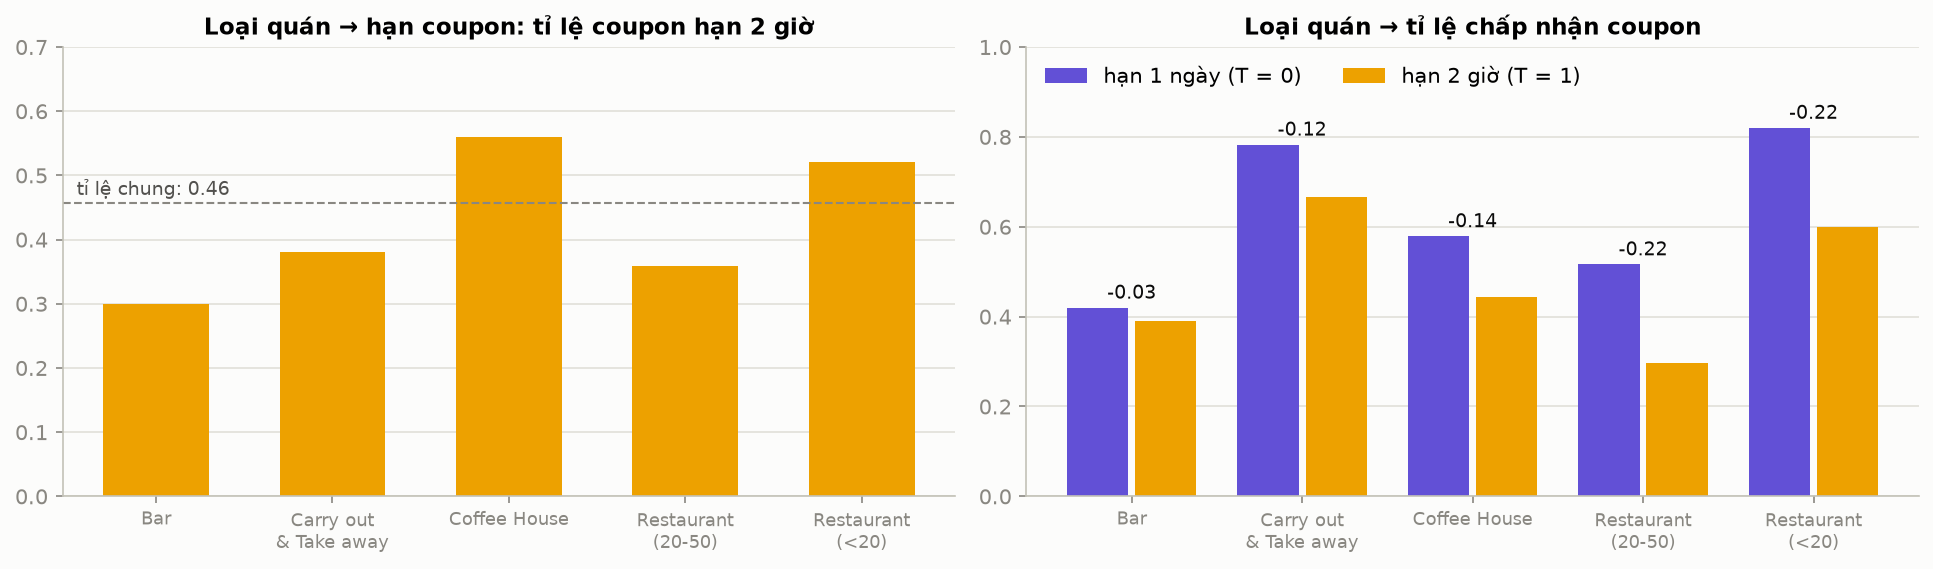
\includegraphics[width=\textwidth]{figures/confounding_by_coupon.png}
\caption{Loại quán là confounder (TRAIN, seed 0). Trái: tỉ lệ coupon hạn 2 giờ theo loại quán. Phải: tỉ lệ chấp nhận theo loại quán và hạn; số trên mỗi cặp cột là hiệu 2 giờ trừ 1 ngày trong loại quán đó.}\label{fig:confounding}
\end{figure}

\subsection{Cấu trúc học được và nhận diện}\label{sec:structure}

Bảng~\ref{tab:structure} liệt kê cấu hình mà VALIDATION chọn ở từng lần chạy; Hình~\ref{fig:dagb0} và~\ref{fig:dagh2} vẽ hai DAG của seed 0.

\begin{table}[t]
\caption{Cấu trúc được VALIDATION chọn. H1 dùng DAG của B0. Viết tắt: Cf = \var{CoffeeHouse}, Co = \var{coupon}, De = \var{destination}, Di = \var{direction\_same}, We = \var{weather}.}\label{tab:structure}
\begin{tabular}{@{}cllclc@{}}
\toprule
Seed & Mô hình & Cấu hình được chọn & Số cạnh & Parents của $Y$ ngoài $T$ & Số parents của $T$ \\
\midrule
0 & B0, H1 & K2, $\le$ 6 parents & 62 & Cf, Co, De, Di & 6 \\
0 & H2 & $\tau$ = 0{,}15 & 40 & Cf, Co, De, We & 7 \\
1 & B0, H1 & K2, $\le$ 6 parents & 62 & Cf, Co, De, Di & 6 \\
1 & H2 & $\tau$ = 0{,}15 & 37 & Cf, Co, De, We & 7 \\
2 & B0, H1 & K2, $\le$ 4 parents & 51 & Cf, Co, De & 4 \\
2 & H2 & $\tau$ = 0{,}15 & 43 & Cf, Co, De, We & 7 \\
3 & B0, H1 & BIC, $\le$ 4 parents & 47 & Cf, Co & 4 \\
3 & H2 & $\tau$ = 0{,}15 & 40 & Cf, Co, De, We & 7 \\
4 & B0, H1 & K2, $\le$ 4 parents & 51 & Cf, Co, De & 4 \\
4 & H2 & $\tau$ = 0{,}10 & 45 & Cf, Co, De, We & 7 \\
\botrule
\end{tabular}
\footnotetext{B0: hàm điểm và số parents tối đa mỗi nút. H2: ngưỡng $\tau$ giữ cạnh.}
\end{table}

\begin{itemize}
\item \textbf{Tuân thủ ràng buộc.} Cả 15 mô hình (3 mô hình $\times$ 5 seed) đều qua \texttt{check\_dag}; không có vi phạm luật hay chu trình nào trong DAG cuối.
\item \textbf{B0.} VALIDATION chọn K2 ở 4/5 seed và BIC ở seed 3. $Y$ luôn có parents $T$, \var{coupon} và \var{CoffeeHouse}; \var{destination} có thêm ở 4/5 seed, \var{direction\_same} ở 2/5 seed. Ở seed 0, DAG có 62 cạnh: 32 cạnh giữa các biến của người trả lời, 18 cạnh giữa các biến kịch bản, 6 cạnh vào $T$, 5 cạnh vào $Y$ và một cạnh $\var{has\_children} \to \var{passenger}$.
\item \textbf{H2.} Ngưỡng $\tau=0{,}15$ được chọn ở seed 0--3 và $\tau=0{,}10$ ở seed 4. Cạnh $T \to Y$ vượt ngưỡng ở cả 5 seed, tức NOTEARS tự tìm ra nó mà không cần luật 10 ép vào. $Y$ có \emph{cùng một} tập parents ở cả 5 seed: $T$, \var{coupon}, \var{CoffeeHouse}, \var{destination}, \var{weather}.
\item \textbf{Thói quen.} Trong năm thói quen gốc, chỉ \var{CoffeeHouse} trở thành parent của $Y$, và nó có mặt ở cả 15 mô hình.
\item \textbf{Parents của $T$.} H2 giữ đủ 7 biến kịch bản ở cả 5 seed; B0 giữ 6 biến ở seed 0, 1 và 4 biến (\var{coupon}, \var{destination}, \var{dist}, \var{weather}) ở ba seed còn lại. Hai cách học đồng ý rằng hạn coupon gắn với kịch bản.
\item \textbf{B0 so với H2 ở seed 0.} H2 có 40 cạnh, B0 có 62: 29 cạnh chung, 33 cạnh chỉ B0 có, 11 cạnh chỉ H2 có. Khác biệt chủ yếu ở phần nối các đặc điểm của người trả lời với nhau (B0: 32 cạnh, H2: 15 cạnh); phần mà câu hỏi cần thì giống nhau. Cạnh $\var{has\_children} \to \var{passenger}$ có ở cả 5 DAG của B0 và ở 3/5 DAG của H2 (seed 2, 3, 4).
\end{itemize}

\begin{figure}[t]
\centering
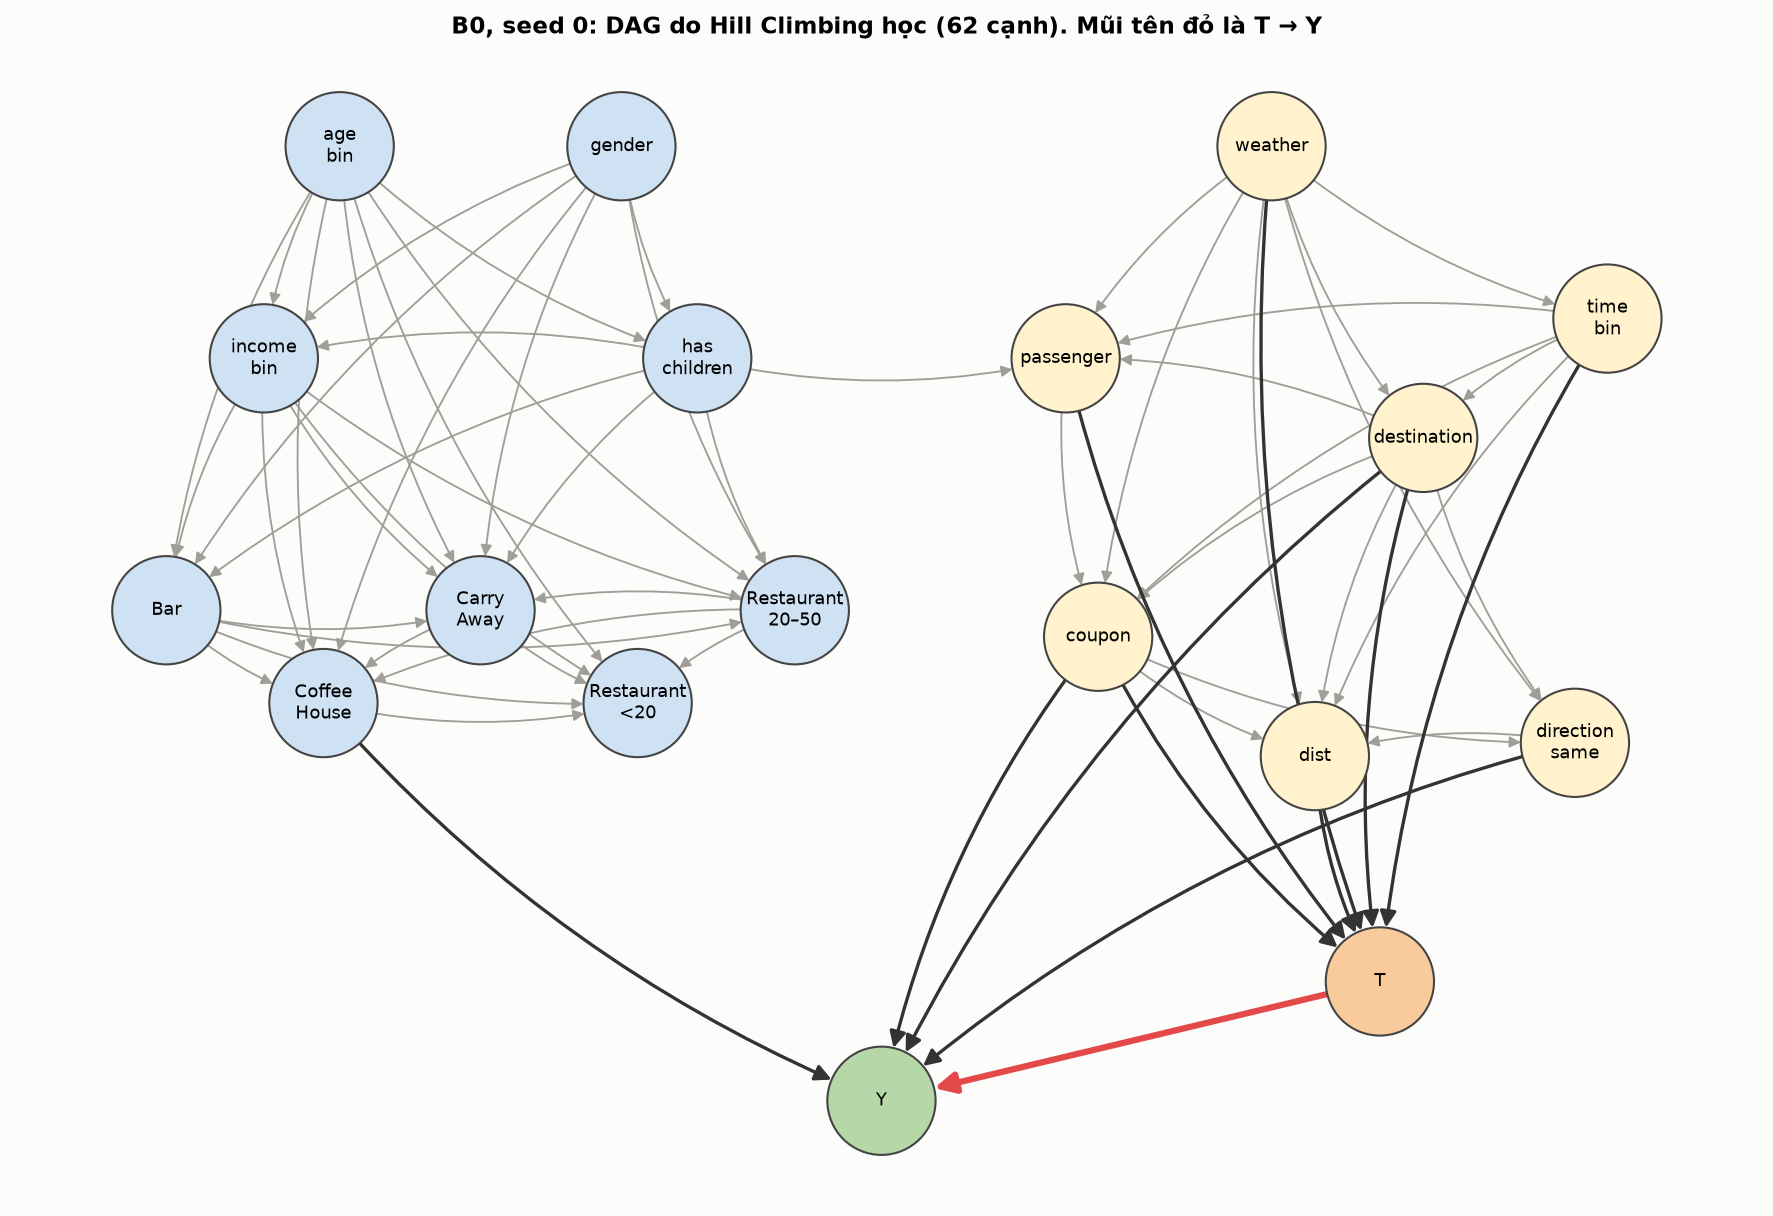
\includegraphics[width=\textwidth]{figures/dag_b0_seed0.png}
\caption{DAG của B0 ở seed 0 (Hill Climbing, điểm K2, tối đa 6 parents; 62 cạnh). Nửa trái: biến của người trả lời; nửa phải: biến kịch bản. Mũi tên vào $T$ hoặc $Y$ vẽ đậm vì chúng quyết định tập điều chỉnh; $T \to Y$ tô đỏ.}\label{fig:dagb0}
\end{figure}

\begin{figure}[t]
\centering
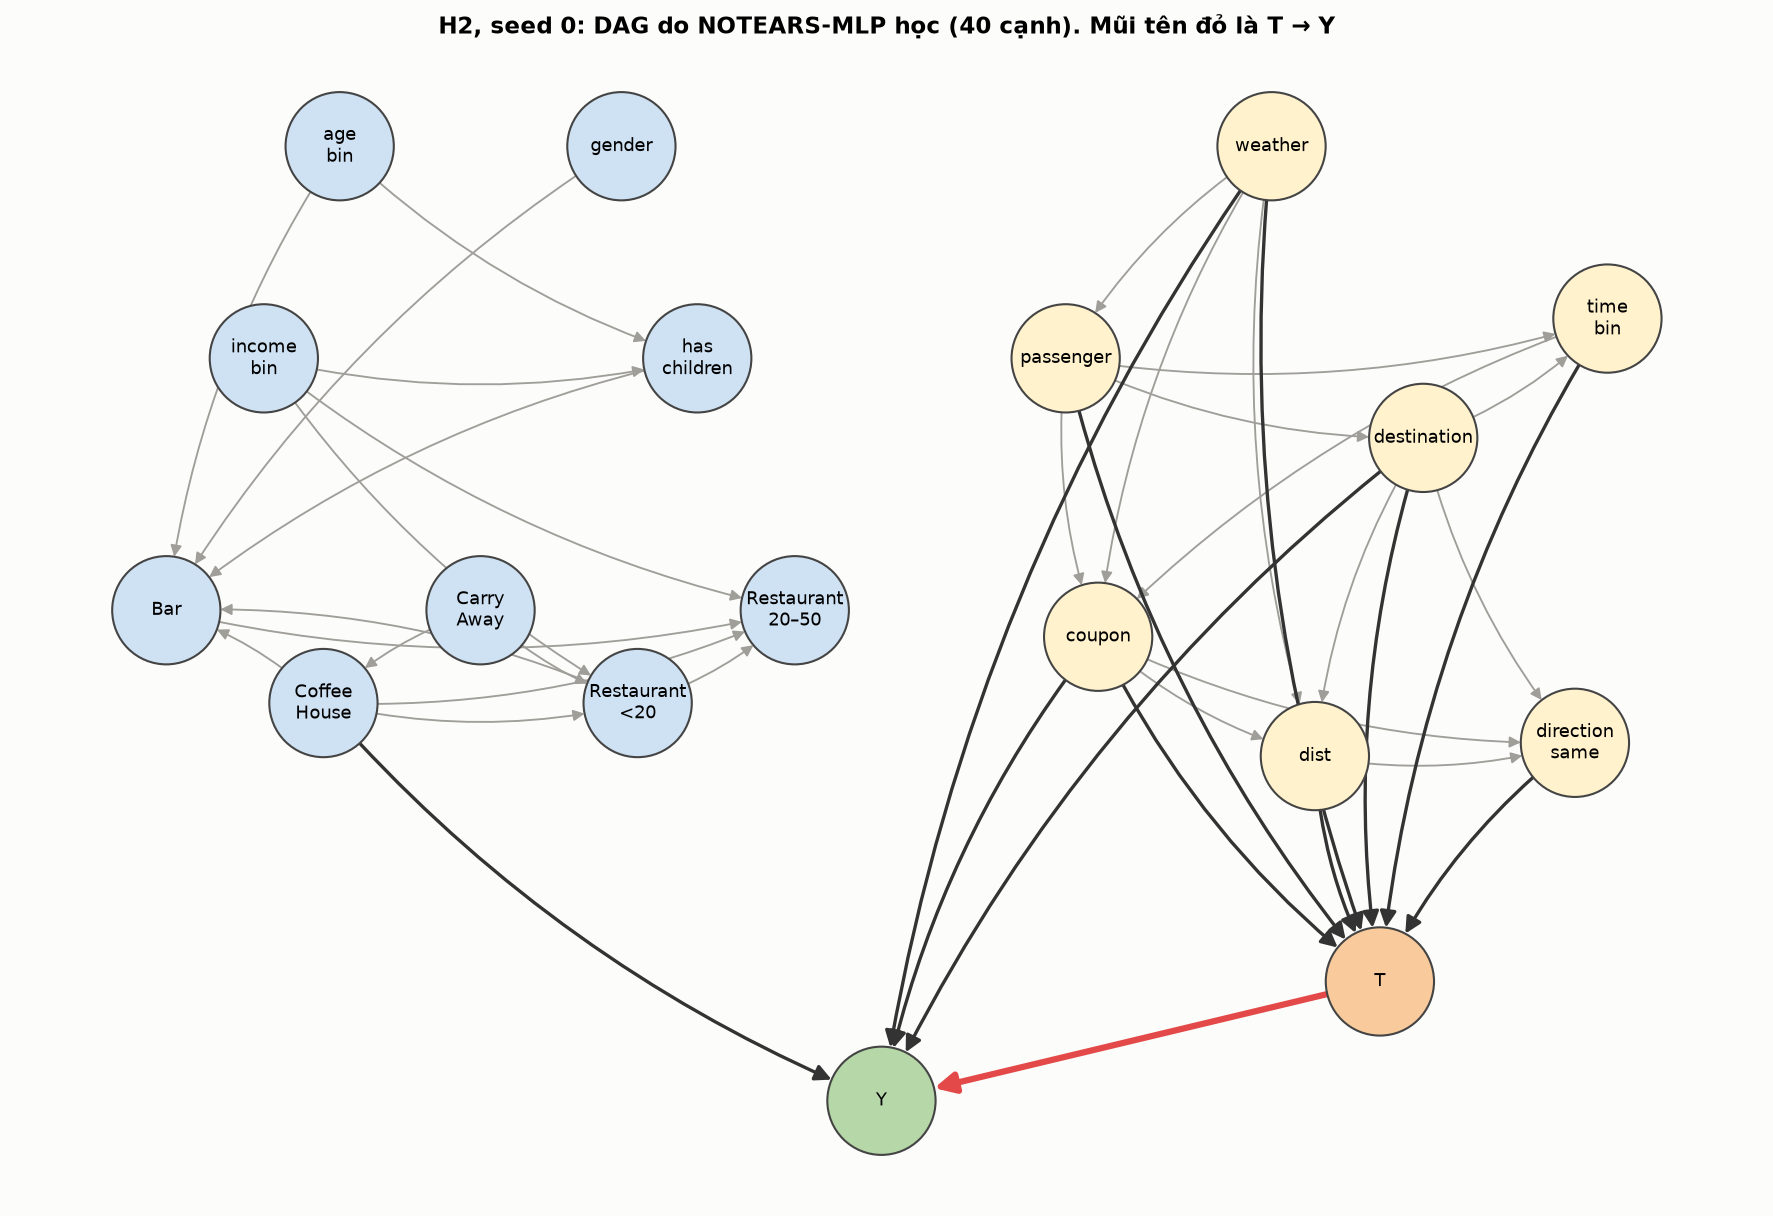
\includegraphics[width=\textwidth]{figures/dag_h2_seed0.png}
\caption{DAG của H2 ở seed 0 (NOTEARS-MLP, ngưỡng 0,15; 40 cạnh). Ở seed này H2 không giữ cạnh $\var{has\_children} \to \var{passenger}$, nên nhóm người trả lời và nhóm kịch bản chỉ gặp nhau ở $Y$.}\label{fig:dagh2}
\end{figure}

\textbf{Chọn mô hình ở seed 0.} Với B0, ứng viên được chọn có log loss của $Y$ trên VALIDATION là 0,598; các ứng viên BIC và BDeu chỉ cho $Y$ hai parents ngoài $T$ và đạt 0,620. Thuật toán PC (kiểm định chi-square, mức 0,01) được chạy một lần để so sánh hai họ thuật toán nhưng không tham gia chọn mô hình: nó chỉ giữ 16 cạnh, cho $Y$ một parent duy nhất là $T$, và có log loss kém nhất (0,672). Với H2, NOTEARS dừng sau 7 vòng ngoài khi $h \approx 3{,}8\times10^{-6}$; ngưỡng 0,15 cho log loss 0,601, tốt hơn ngưỡng 0,10 (0,619) và 0,20 (0,638).

\textbf{Nhận diện.} DoWhy nhận diện được hiệu ứng bằng tiêu chí backdoor trên cả 10 DAG (5 của B0, 5 của H2); không có trường hợp không nhận diện được. Mọi tập điều chỉnh, của DoWhy lẫn của mô hình, đều chặn hết backdoor path theo kiểm tra d-separation. Hai tập thường khác nhau ở một biến mà vẫn cùng hợp lệ. Ví dụ ở seed 0 trên DAG của B0, DoWhy chọn \{\var{coupon}, \var{destination}, \var{direction\_same}, \var{has\_children}\} còn mô hình dùng \{\var{coupon}, \var{destination}, \var{direction\_same}, \var{CoffeeHouse}\}: cả hai cùng chặn đường $T \leftarrow \var{passenger} \leftarrow \var{has\_children} \to \cdots \to \var{CoffeeHouse} \to Y$, một bên chặn ở \var{has\_children}, một bên ở \var{CoffeeHouse}. Ở cả 10 DAG, tập của DoWhy không chứa \var{CoffeeHouse}; điều này khớp với bộ luật, vì thói quen chỉ có thể nối với $T$ qua cạnh $\var{has\_children} \to \var{passenger}$. Phép ``ép $T$ rồi tra bảng'' trùng với \texttt{do()} của \texttt{pgmpy} ở cả 15 mô hình (lệch lớn nhất $1{,}1\times10^{-16}$).

\subsection{Bảng A: dự đoán trên TEST}\label{sec:tableA}

\begin{table}[t]
\caption{\textbf{Table A.1.} Dự đoán $Y$ trên TEST, từng lần chạy và tóm tắt. $n$: số dòng TEST. Ngưỡng: ngưỡng macro-F1 chọn trên VALIDATION. Học: thời gian học (giây).}\label{tab:A1}
\setlength{\tabcolsep}{2.6pt}
\begin{tabular}{@{}cclcccccc@{}}
\toprule
Seed & $n$ & Mô hình & AUROC $\uparrow$ & macro-F1 $\uparrow$ & Brier $\downarrow$ & Log loss $\downarrow$ & Ngưỡng & Học \\
\midrule
0 & 1.855 & B0 & 0,734 & 0,669 & 0,204 & 0,601 & 0,59 & 2,9 \\
 &  & H1 & 0,738 & 0,666 & 0,203 & 0,592 & 0,59 & 0,6 \\
 &  & H2 & 0,729 & 0,672 & 0,207 & 0,616 & 0,53 & 34,0 \\
\addlinespace[2pt]
1 & 1.810 & B0 & 0,728 & 0,684 & 0,207 & 0,616 & 0,56 & 2,4 \\
 &  & H1 & 0,736 & 0,683 & 0,205 & 0,598 & 0,60 & 0,3 \\
 &  & H2 & 0,731 & 0,680 & 0,208 & 0,622 & 0,50 & 14,7 \\
\addlinespace[2pt]
2 & 1.799 & B0 & 0,718 & 0,661 & 0,209 & 0,612 & 0,53 & 4,6 \\
 &  & H1 & 0,726 & 0,668 & 0,206 & 0,600 & 0,64 & 0,5 \\
 &  & H2 & 0,723 & 0,670 & 0,210 & 0,631 & 0,59 & 35,2 \\
\addlinespace[2pt]
3 & 1.813 & B0 & 0,692 & 0,633 & 0,218 & 0,625 & 0,53 & 2,8 \\
 &  & H1 & 0,691 & 0,638 & 0,218 & 0,624 & 0,52 & 0,3 \\
 &  & H2 & 0,724 & 0,665 & 0,209 & 0,611 & 0,51 & 30,7 \\
\addlinespace[2pt]
4 & 1.853 & B0 & 0,756 & 0,698 & 0,197 & 0,588 & 0,62 & 2,8 \\
 &  & H1 & 0,764 & 0,706 & 0,196 & 0,577 & 0,60 & 0,3 \\
 &  & H2 & 0,760 & 0,705 & 0,197 & 0,602 & 0,52 & 31,7 \\
\midrule
\multicolumn{2}{@{}l}{TB $\pm$ ĐLC} & B0 & 0,726 $\pm$ 0,023 & 0,669 $\pm$ 0,025 & 0,207 $\pm$ 0,008 & 0,608 $\pm$ 0,014 & & 3,1 \\
\multicolumn{2}{@{}l}{TB $\pm$ ĐLC} & H1 & 0,731 $\pm$ 0,026 & 0,672 $\pm$ 0,025 & 0,205 $\pm$ 0,008 & 0,598 $\pm$ 0,017 & & 0,4 \\
\multicolumn{2}{@{}l}{TB $\pm$ ĐLC} & H2 & 0,733 $\pm$ 0,015 & 0,678 $\pm$ 0,016 & 0,206 $\pm$ 0,005 & 0,617 $\pm$ 0,011 & & 29,3 \\
\botrule
\end{tabular}
\footnotetext{TB $\pm$ ĐLC: trung bình và độ lệch chuẩn qua 5 seed. Tỉ lệ $Y{=}1$ trên TEST: 0,584; 0,569; 0,580; 0,584; 0,575 (seed 0--4). Thời gian học của B0 gồm sáu lần Hill Climbing và bước chọn; của H1 chỉ gồm huấn luyện MLP (DAG lấy từ B0); của H2 gồm NOTEARS và bước chọn ngưỡng.}
\end{table}

\begin{table}[t]
\caption{\textbf{Table A.2.} Hiệu theo cặp so với B0 (cùng seed). Với AUROC và macro-F1, hiệu dương là tốt hơn B0; với Brier và log loss, hiệu âm là tốt hơn B0.}\label{tab:A2}
\begin{tabular}{@{}llccccc@{}}
\toprule
Chỉ số & So sánh & Hiệu trung bình & ĐLC & Nhỏ nhất & Lớn nhất & Số seed hiệu $>0$ \\
\midrule
AUROC & H1 $-$ B0 & 0,0053 & 0,0038 & $-$0,0007 & 0,0083 & 4/5 \\
AUROC & H2 $-$ B0 & 0,0076 & 0,0142 & $-$0,0053 & 0,0319 & 4/5 \\
macro-F1 & H1 $-$ B0 & 0,0032 & 0,0050 & $-$0,0030 & 0,0076 & 3/5 \\
macro-F1 & H2 $-$ B0 & 0,0092 & 0,0136 & $-$0,0046 & 0,0317 & 4/5 \\
Brier & H1 $-$ B0 & $-$0,0019 & 0,0010 & $-$0,0030 & $-$0,0004 & 0/5 \\
Brier & H2 $-$ B0 & $-$0,0012 & 0,0047 & $-$0,0094 & 0,0027 & 3/5 \\
Log loss & H1 $-$ B0 & $-$0,0103 & 0,0064 & $-$0,0184 & $-$0,0008 & 0/5 \\
Log loss & H2 $-$ B0 & 0,0082 & 0,0132 & $-$0,0138 & 0,0191 & 4/5 \\
\botrule
\end{tabular}
\end{table}

Mốc so sánh ở seed 0: luôn dự đoán bằng tỉ lệ chung 0,576 cho AUROC 0,5 và Brier 0,243. Cả ba mô hình đều học được quy luật nhưng còn xa mức hoàn hảo, hợp lý vì quyết định nhận coupon phụ thuộc nhiều thứ không có trong dữ liệu. Từ Bảng~\ref{tab:A1} và~\ref{tab:A2}:

\begin{itemize}
\item \textbf{Ba mô hình xếp hạng gần ngang nhau:} AUROC trung bình 0,726 (B0), 0,731 (H1), 0,733 (H2). Log loss thì có khác: 0,608 (B0), 0,598 (H1), 0,617 (H2).
\item \textbf{H1 so với B0:} log loss và Brier của H1 thấp hơn ở cả 5/5 seed (log loss trung bình $-$0,010, ĐLC 0,006); AUROC cao hơn ở 4/5 seed (+0,005). Mức hơn nhỏ nhưng cùng chiều; ở seed 3 hai mô hình gần như bằng nhau. MLP cho xác suất sát hơn một chút, chưa đủ để nói là hơn hẳn.
\item \textbf{H2 so với B0:} AUROC cao hơn ở 4/5 seed (trung bình +0,008), nhưng phần lớn mức hơn đến từ seed 3 (+0,032), nơi B0 chỉ cho $Y$ hai parents ngoài $T$; ở seed 0 H2 kém B0 ($-$0,005). Log loss thì ngược lại: kém B0 ở 4/5 seed (trung bình +0,008), chỉ hơn ở seed 3. H2 xếp hạng ngang hoặc nhỉnh hơn, nhưng xác suất kém chính xác hơn vì bảng CPD 360 ô của $Y$ có nhiều ô ít dữ liệu.
\item \textbf{Chênh lệch giữa các seed lớn hơn chênh lệch giữa các mô hình:} ĐLC của AUROC qua các seed là 0,016 đến 0,026, còn hiệu giữa các mô hình là 0,005 đến 0,008. Nếu chỉ chạy một seed thì rất dễ kết luận nhầm.
\end{itemize}

Hình~\ref{fig:h1} minh hoạ H1 ở seed 0: mạng có 1.089 tham số, học 79 epoch và giữ lại mạng ở epoch 68 (log loss trên VALIDATION 0,596). Ở các ô có nhiều dữ liệu, bảng đếm và MLP đồng ý với nhau; ở 71 ô không có dòng TRAIN nào, B0 trả về 0,5 còn H1 đưa ra một dự đoán dựa trên các ô tương tự.

\begin{figure}[t]
\centering
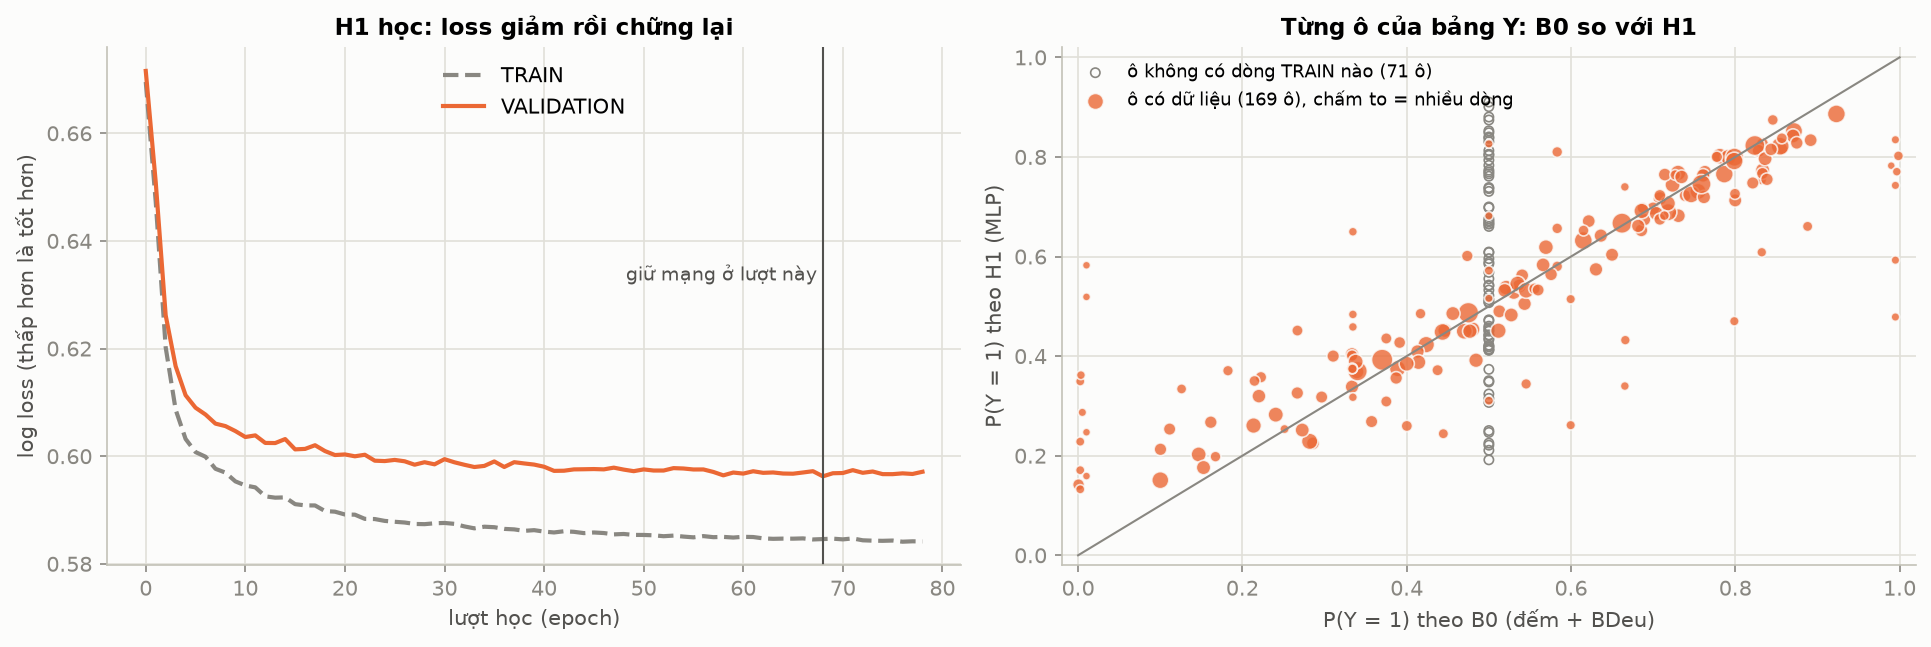
\includegraphics[width=\textwidth]{figures/h1_seed0.png}
\caption{H1 ở seed 0. Trái: log loss trên TRAIN và VALIDATION theo epoch; vạch dọc là epoch được giữ lại. Phải: từng ô của CPD của $Y$, B0 (trục ngang) so với H1 (trục dọc); vòng tròn rỗng là 71 ô không có dòng TRAIN nào.}\label{fig:h1}
\end{figure}

Các chỉ số trên đo khả năng dự đoán $Y$ quan sát được. Dự đoán tốt hơn không xác nhận ATE đúng hơn; Bảng A và Bảng B trả lời hai câu hỏi khác nhau.

\subsection{Bảng B: can thiệp trên nhóm tham chiếu TEST}\label{sec:tableB}

\begin{table}[t]
\caption{\textbf{Table B.1.} Can thiệp trên nhóm tham chiếu TEST của từng seed (kích thước ở Bảng~\ref{tab:A1}). Control: $T=0$ (1 ngày); treatment: $T=1$ (2 giờ). Công thức nhận diện: backdoor~\eqref{eq:backdoor} với tập điều chỉnh $Z$; ước lượng theo~\eqref{eq:std}.}\label{tab:B1}
\setlength{\tabcolsep}{3pt}
\begin{tabular}{@{}clccccL{2.0cm}c@{}}
\toprule
Seed & Mô hình & risk(1 ngày) & risk(2 giờ) & ATE & CI 95\% & Tập điều chỉnh $Z$ & Ô trống (\%) \\
\midrule
0 & B0 & 0,636 & 0,487 & $-$0,149 & [$-$0,170; $-$0,122] & Cf, Co, De, Di & 2,9 \\
 & H1 & 0,637 & 0,487 & $-$0,150 & [$-$0,168; $-$0,127] & Cf, Co, De, Di & 2,9 \\
 & H2 & 0,631 & 0,496 & $-$0,135 & [$-$0,162; $-$0,108] & Cf, Co, De, We & 13,5 \\
\addlinespace[2pt]
1 & B0 & 0,639 & 0,489 & $-$0,150 & [$-$0,169; $-$0,131] & Cf, Co, De, Di & 2,8 \\
 & H1 & 0,647 & 0,490 & $-$0,158 & [$-$0,175; $-$0,141] & Cf, Co, De, Di & 2,8 \\
 & H2 & 0,632 & 0,488 & $-$0,145 & [$-$0,161; $-$0,126] & Cf, Co, De, We & 14,9 \\
\addlinespace[2pt]
2 & B0 & 0,653 & 0,494 & $-$0,158 & [$-$0,177; $-$0,132] & Cf, Co, De & 0,0 \\
 & H1 & 0,664 & 0,508 & $-$0,156 & [$-$0,178; $-$0,133] & Cf, Co, De & 0,0 \\
 & H2 & 0,648 & 0,501 & $-$0,147 & [$-$0,164; $-$0,119] & Cf, Co, De, We & 13,7 \\
\addlinespace[2pt]
3 & B0 & 0,636 & 0,477 & $-$0,159 & [$-$0,182; $-$0,138] & Cf, Co & 0,0 \\
 & H1 & 0,628 & 0,476 & $-$0,151 & [$-$0,170; $-$0,129] & Cf, Co & 0,0 \\
 & H2 & 0,635 & 0,482 & $-$0,153 & [$-$0,174; $-$0,132] & Cf, Co, De, We & 14,1 \\
\addlinespace[2pt]
4 & B0 & 0,658 & 0,487 & $-$0,171 & [$-$0,189; $-$0,147] & Cf, Co, De & 0,6 \\
 & H1 & 0,650 & 0,491 & $-$0,159 & [$-$0,176; $-$0,130] & Cf, Co, De & 0,6 \\
 & H2 & 0,649 & 0,491 & $-$0,158 & [$-$0,176; $-$0,134] & Cf, Co, De, We & 15,3 \\
\botrule
\end{tabular}
\footnotetext{CI 95\%: bootstrap phân vị, 100 lần, rút theo người trên TRAIN, DAG và nhóm TEST cố định. Ô trống: tỉ lệ dòng TEST cần ít nhất một ô CPD không có dòng TRAIN nào khi can thiệp. Viết tắt như Bảng~\ref{tab:structure}. Mọi DAG đều hợp lệ và mọi tập $Z$ đều thoả tiêu chí backdoor.}
\end{table}

\begin{table}[t]
\caption{\textbf{Table B.2.} Tóm tắt qua 5 seed (trung bình $\pm$ ĐLC) và hiệu ATE theo cặp so với B0. ATE DoWhy: ước lượng tham chiếu bằng hồi quy tuyến tính trên DAG của mô hình (H1 dùng DAG của B0).}\label{tab:B2}
\begin{tabular}{@{}lccccc@{}}
\toprule
Mô hình & risk(1 ngày) & risk(2 giờ) & ATE & ATE DoWhy & Ô trống (\%) \\
\midrule
B0 & 0,644 $\pm$ 0,010 & 0,487 $\pm$ 0,006 & $-$0,157 $\pm$ 0,009 & $-$0,164 $\pm$ 0,005 & 1,3 \\
H1 & 0,645 $\pm$ 0,014 & 0,490 $\pm$ 0,011 & $-$0,155 $\pm$ 0,004 & $-$0,164 $\pm$ 0,005 & 1,3 \\
H2 & 0,639 $\pm$ 0,009 & 0,492 $\pm$ 0,007 & $-$0,148 $\pm$ 0,009 & $-$0,165 $\pm$ 0,005 & 14,3 \\
\botrule
\end{tabular}

\vspace{6pt}
\begin{tabular}{@{}llccccc@{}}
\toprule
Chỉ số & So sánh & Hiệu trung bình & ĐLC & Nhỏ nhất & Lớn nhất & Số seed hiệu $>0$ \\
\midrule
ATE & H1 $-$ B0 & 0,0023 & 0,0077 & $-$0,0082 & 0,0116 & 3/5 \\
ATE & H2 $-$ B0 & 0,0098 & 0,0042 & 0,0048 & 0,0140 & 5/5 \\
\botrule
\end{tabular}
\end{table}

\begin{figure}[t]
\centering
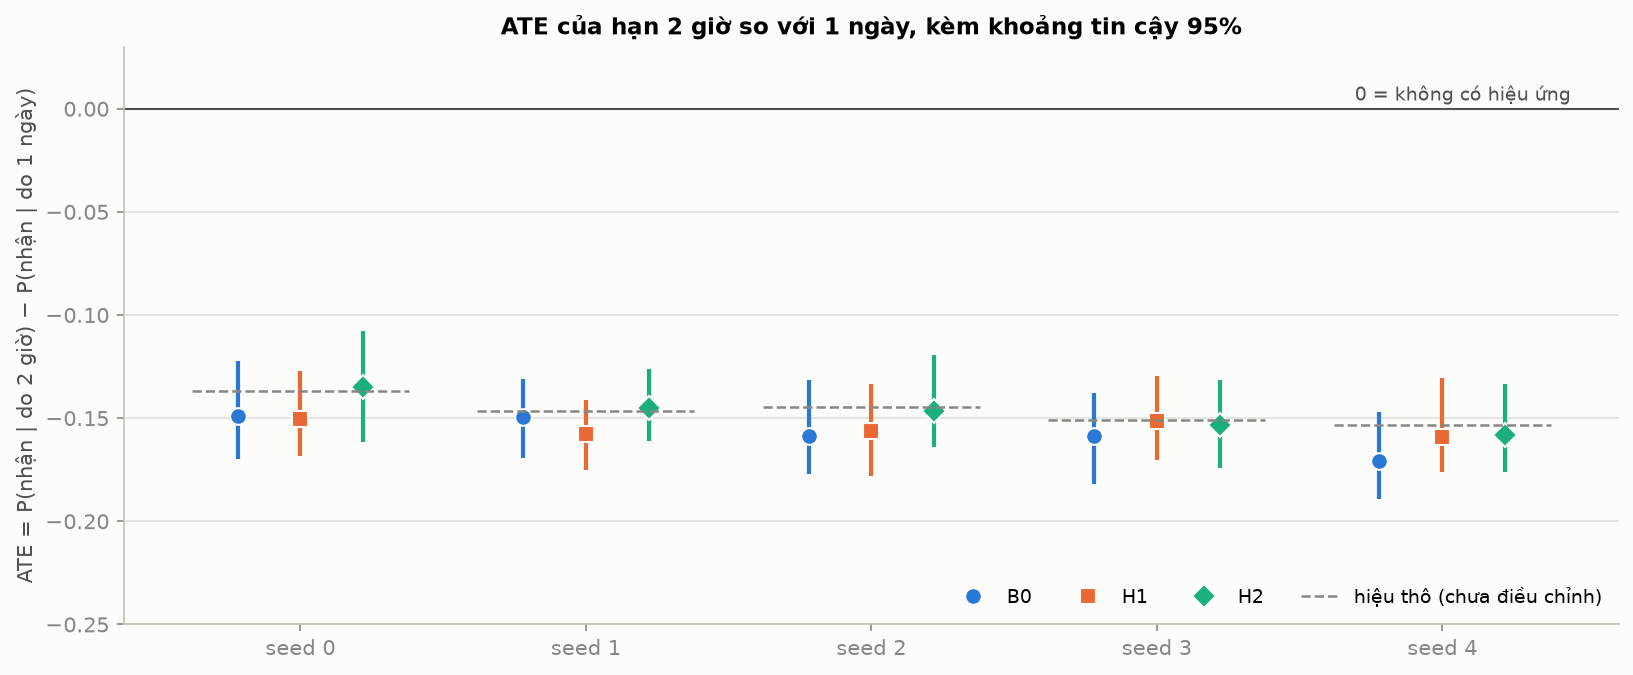
\includegraphics[width=\textwidth]{figures/ate_by_seed.png}
\caption{ATE của ba mô hình ở từng seed kèm CI 95\%. Vạch xám đứt là hiệu thô trên TRAIN, chưa điều chỉnh.}\label{fig:ate}
\end{figure}

\begin{itemize}
\item \textbf{Câu trả lời.} Nếu mọi coupon có hạn 1 ngày, khoảng 64\% được chấp nhận; nếu mọi coupon có hạn 2 giờ, khoảng 49\%. ATE trung bình là $-$0,157 (B0), $-$0,155 (H1) và $-$0,148 (H2).
\item \textbf{Độ bất định.} Cả 15 CI 95\% nằm hẳn dưới 0 (Hình~\ref{fig:ate}). Nửa độ rộng trung bình của CI là khoảng 0,02 với cả ba mô hình.
\item \textbf{Ba mô hình gần nhau.} Hiệu ATE theo cặp là +0,002 (H1 $-$ B0) và +0,010 (H2 $-$ B0), nhỏ so với độ rộng của CI. Hiệu của H1 đổi dấu giữa các seed (3/5 dương). Riêng H2 lệch \emph{cùng một chiều} ở cả 5/5 seed: ATE của nó gần 0 hơn B0 từ 0,005 đến 0,014.
\item \textbf{Vì sao H2 gần 0 hơn.} Nhiều khả năng do ô trống: ở cả 5 seed, 13,5--15,3\% dòng TEST của H2 phải dùng một ô không có dòng TRAIN nào (B0 và H1: không quá 2,9\%), vì \var{weather} có hai mức ít dòng (Rainy, Snowy). Ô trống có giá trị 0,5 ở cả hai loại hạn nên kéo hiệu về 0. Con số của H2 vì thế cần đọc thận trọng hơn.
\item \textbf{Đối chiếu.} Hiệu thô trên TRAIN trung bình là $-$0,146. Ước lượng độc lập của DoWhy (hồi quy tuyến tính) cho $-$0,164 trên DAG của B0 và $-$0,165 trên DAG của H2, cùng cỡ với ba mô hình; phép tính tay ở seed 0 cho $-$0,152.
\end{itemize}

\textbf{Giới hạn khi đọc Bảng B.} CI của từng seed có điều kiện trên DAG, tập VALIDATION và nhóm TEST cố định; nó không gồm sai DAG, thiếu overlap hay bất định của quần thể TEST. Trung bình các đầu mút CI qua seed chỉ là mô tả, không phải CI 95\% của một ATE tổng hợp. Hiệu thô trên TRAIN và ATE chuẩn hoá trên TEST khác nhau cả do thành phần mẫu lẫn do cách ước lượng, nên không quy toàn bộ chênh lệch cho confounding đã được sửa.

\subsection{Bảng C: độ ổn định, độ vững và chi phí}\label{sec:tableC}

\begin{table}[t]
\caption{\textbf{Table C.1.} Độ ổn định qua 5 lần chạy. Số tập $\PaY$: số tập parents của $Y$ khác nhau qua 5 seed. Hai cột cuối: số seed có ATE $<0$ và số seed có CI 95\% không chứa 0.}\label{tab:C1}
\setlength{\tabcolsep}{4pt}
\begin{tabular}{@{}lcccccccc@{}}
\toprule
 & Số cạnh & Số tập & \multicolumn{4}{c}{ATE qua 5 seed} & ATE & CI \\
\cmidrule(lr){4-7}
Mô hình & (min--max) & $\PaY$ & TB & ĐLC & Nhỏ nhất & Lớn nhất & $<0$ & $\not\ni 0$ \\
\midrule
B0 & 47--62 & 3 & $-$0,1573 & 0,0089 & $-$0,1709 & $-$0,1488 & 5/5 & 5/5 \\
H1 & 47--62 & 3 & $-$0,1550 & 0,0040 & $-$0,1593 & $-$0,1503 & 5/5 & 5/5 \\
H2 & 37--45 & 1 & $-$0,1475 & 0,0089 & $-$0,1583 & $-$0,1348 & 5/5 & 5/5 \\
\botrule
\end{tabular}
\end{table}

\begin{table}[t]
\caption{\textbf{Table C.2.} Hai refuter của DoWhy trên ước lượng hồi quy tuyến tính (100 lần mô phỏng mỗi phép thử, seed của refuter bằng seed của lần chạy). Cả 20 phép thử đều đạt tiêu chí khai báo trước.}\label{tab:C2}
\setlength{\tabcolsep}{3.5pt}
\begin{tabular}{@{}cllccccc@{}}
\toprule
 & & & & \multicolumn{2}{c}{Placebo treatment} & \multicolumn{2}{c}{Data subset (80\%)} \\
\cmidrule(lr){5-6}\cmidrule(lr){7-8}
Seed & DAG & Tập điều chỉnh DoWhy & ATE DoWhy & Hiệu ứng mới & $p$ & Hiệu ứng mới & $p$ \\
\midrule
0 & B0 & Co, De, Di, Hc & $-$0,1578 & $-$0,0009 & 0,96 & $-$0,1581 & 0,94 \\
 & H2 & Co, De, We & $-$0,1594 & $-$0,0009 & 0,98 & $-$0,1597 & 0,92 \\
1 & B0 & Co, De, Di, Hc & $-$0,1657 & 0,0001 & 0,92 & $-$0,1654 & 0,92 \\
 & H2 & Co, De, We & $-$0,1664 & 0,0003 & 0,96 & $-$0,1660 & 0,88 \\
2 & B0 & Co, De, We & $-$0,1623 & 0,0020 & 0,84 & $-$0,1629 & 0,84 \\
 & H2 & Co, De, Hc, We & $-$0,1613 & 0,0020 & 0,86 & $-$0,1618 & 0,82 \\
3 & B0 & Co, Hc & $-$0,1624 & 0,0006 & 0,88 & $-$0,1629 & 0,94 \\
 & H2 & Co, De, Hc, We & $-$0,1678 & 0,0004 & 0,94 & $-$0,1684 & 0,94 \\
4 & B0 & Co, De, We & $-$0,1723 & 0,0014 & 0,88 & $-$0,1722 & 1,00 \\
 & H2 & Co, De, Hc, We & $-$0,1715 & 0,0014 & 0,86 & $-$0,1714 & 0,96 \\
\botrule
\end{tabular}
\footnotetext{Viết tắt như Bảng~\ref{tab:structure}; Hc = \var{has\_children}. Kết quả trên DAG của B0 cũng áp cho H1 vì hai mô hình dùng chung DAG.}
\end{table}

\begin{table}[t]
\caption{\textbf{Table C.3 và C.4.} Placebo trên chính mô hình (20 lần hoán vị $T$ mỗi seed) và chi phí tính toán (trung bình 5 seed).}\label{tab:C3}
\begin{tabular}{@{}lccccc@{}}
\toprule
 & ATE thật & ATE placebo & $|\text{ATE placebo}|$ & Thời gian học & Truy vấn $\doop()$ trên \\
Mô hình & (TB) & (TB) & lớn nhất & (giây) & TEST (ms) \\
\midrule
B0 & $-$0,1573 & $-$0,0010 & 0,0347 & 3,1 & 2,8 \\
H1 & $-$0,1550 & $-$0,0005 & 0,0228 & 0,4 & 2,8 \\
H2 & $-$0,1475 & $-$0,0011 & 0,0353 & 29,3 & 3,1 \\
\botrule
\end{tabular}
\footnotetext{Phần cứng: macOS trên CPU ARM 8 lõi, không GPU. Dự đoán và truy vấn can thiệp đều là tra bảng CPD của $Y$; thời gian dự đoán không được đo riêng.}
\end{table}

\begin{itemize}
\item \textbf{C.1 Ổn định.} Với cả ba mô hình, ATE âm ở 5/5 seed và CI không chứa 0 ở 5/5 seed. ĐLC của ATE qua các seed là 0,009 (B0), 0,004 (H1), 0,009 (H2), nhỏ so với độ lớn 0,15--0,16 của hiệu ứng. Về cấu trúc, qua 5 seed B0 cho 3 tập parents của $Y$ khác nhau còn H2 chỉ cho một. ATE của B0 vẫn gần như không đổi vì \var{coupon} và \var{CoffeeHouse} luôn có mặt.
\item \textbf{C.2 Refuter của DoWhy.} Đạt ở cả 10 DAG. Với $T$ bị hoán vị, hiệu ứng rơi về trong khoảng $\pm$0,002 (hiệu ứng gốc khoảng $-$0,16). Khi chỉ giữ 80\% dữ liệu, hiệu ứng lệch không quá 0,001. Mọi $p$-value từ 0,82 trở lên.
\item \textbf{C.3 Placebo trên mô hình.} ATE placebo trung bình xấp xỉ 0 (khoảng $-$0,001). Giá trị xa 0 nhất trong các lần hoán vị là 0,035 (B0), 0,023 (H1), 0,035 (H2), vẫn nhỏ hơn ATE thật hơn 4 lần.
\item \textbf{C.4 Chi phí.} Học B0 mất khoảng 3 giây mỗi seed; H1 cần thêm khoảng 0,4 giây để huấn luyện MLP; H2 mất khoảng 29 giây, gấp khoảng 9 lần B0. Truy vấn can thiệp trên cả nhóm TEST mất khoảng 3 mili giây với mọi mô hình.
\end{itemize}

Các phép thử này phát hiện lỗi của \emph{phương pháp ước lượng} (bịa ra hiệu ứng, phụ thuộc vào vài dòng cá biệt). Chúng không phát hiện được confounder bị bỏ sót (G2) và không chứng minh DAG đúng.

\subsection{Kết quả bất lợi và sự cố}\label{sec:failures}

\begin{itemize}
\item \textbf{Ô không được hỗ trợ.} Ở seed 0, CPD của $Y$ trong B0 có 240 ô (120 hoàn cảnh $\times$ 2 loại hạn), trong đó 71 ô không có dòng TRAIN nào; trong 78 hoàn cảnh có dữ liệu cho cả hai loại hạn, 64 hoàn cảnh có xác suất chấp nhận thấp hơn khi hạn 2 giờ. Các ô trống ít khi được dùng với B0 và H1 (0--2,9\% dòng TEST) nhưng thường xuyên với H2 (trung bình 14,3\%). Quần thể mục tiêu không bị thu hẹp thêm; thay vào đó tỉ lệ này được báo cáo cùng ATE.
\item \textbf{Ngưỡng thấp của H2.} Ở seed 0 với $\tau=0{,}05$, $Y$ nhận 9 parents ngoài $T$ và log loss trên VALIDATION vọt lên 1,45: bảng CPD quá lớn so với dữ liệu. VALIDATION loại ứng viên này.
\item \textbf{Ổn định số của NOTEARS.} Ngưỡng dừng $h \le 10^{-8}$ dùng ở phiên bản trước gây lỗi số học (NaN) khi kết hợp với bộ luật chặt; báo cáo này dùng $10^{-5}$. Thay đổi của H2 so với phiên bản trước vì thế có thể đến từ bộ luật, từ ngưỡng dừng, hoặc cả hai; hai yếu tố chưa được tách riêng.
\item \textbf{Seed 3.} B0 chỉ cho $Y$ hai parents ngoài $T$ và có AUROC thấp nhất (0,692); H1 dùng cùng DAG nên không cải thiện được (0,691).
\item \textbf{Tái lập.} Mới có một lượt chạy đầy đủ. Khi một DAG có nhiều tập backdoor hợp lệ, DoWhy có thể trả về tập khác giữa hai lần chạy, nên ATE DoWhy có thể lệch ở chữ số thứ ba; H2 và DoWhy chưa được kiểm tra tái lập qua hai lượt chạy.
\end{itemize}

%% ===================================================================
\section{Kết luận}\label{sec:conclusion}
%% (mục 2.7 của rubric)

\textbf{Đặt hạn coupon 2 giờ thay cho 1 ngày đi kèm xác suất chấp nhận coupon thấp hơn khoảng 15--16 điểm phần trăm: từ khoảng 64\% xuống khoảng 49\%.} Ba mô hình, ước lượng hồi quy của DoWhy và phép tính tay cho kết quả cùng cỡ; hiệu ứng âm ở cả năm cách chia và cả 15 CI 95\% nằm dưới 0.

\textbf{Neural CPD (H1).} Cải thiện dự đoán nhỏ nhưng cùng chiều (log loss thấp hơn B0 ở 5/5 seed, trung bình 0,010) và không làm đổi kết luận can thiệp (ATE lệch +0,002, đổi dấu giữa các seed). ĐLC của ATE qua seed của H1 nhỏ hơn B0 (0,004 so với 0,009), nhưng ổn định hơn không có nghĩa là đúng hơn.

\textbf{Neural discovery (H2).} Cho cấu trúc quanh $Y$ ổn định hơn (một tập parents ở cả 5 seed, so với 3 của B0) và tự tìm ra cạnh $T \to Y$, nhưng không cải thiện log loss (kém B0 ở 4/5 seed) và tốn thời gian gấp khoảng 9 lần. ATE của nó gần 0 hơn B0 ở 5/5 seed, nhiều khả năng do ô CPD trống chứ không phải do DAG tốt hơn. Kết luận can thiệp không đổi.

\textbf{Kết quả null.} Thay thành phần truyền thống bằng neural network không làm đổi câu trả lời và không cho lợi ích dự đoán đáng kể trên bộ dữ liệu này. Với 18 biến rời rạc ít mức và khoảng 8.500 dòng TRAIN, bảng đếm làm trơn đã đủ; H1 và H2 đóng vai trò kiểm tra chéo. Nếu chỉ chọn một mô hình thì B0 là đủ.

\subsection{Hạn chế}\label{sec:limits}

\begin{enumerate}
\item \textbf{Không kiểm chứng được G2.} Nếu bảng hỏi gán hạn coupon theo một yếu tố ảnh hưởng $Y$ mà 16 biến nền không ghi lại, ATE sẽ chệch; các refuter không phát hiện được điều này.
\item \textbf{$Y$ là ý định khai trong tình huống giả định,} không phải hành vi thật (G5).
\item \textbf{Bộ luật là hiểu biết đưa vào, không phải kết quả học được.} Nếu một luật sai, DAG và tập điều chỉnh sai theo mà \texttt{check\_dag} không phát hiện được. Chiều của các cạnh trong cùng một nhóm biến không phải quan hệ nhân quả đã xác nhận.
\item \textbf{Dữ liệu nhỏ, CPD thưa.} Chỉ có 587 người trả lời. CI giữ cố định DAG nên chưa gồm độ bất định của việc tìm DAG.
\item \textbf{H2 có hai tham số chưa dò lại trên bộ dữ liệu này:} hệ số phạt L1 cho các cạnh đi vào $T$ ($w_T$) và ngưỡng dừng của $h$.
\item \textbf{Mới có 5 seed và một lượt chạy đầy đủ.} So sánh giữa ba mô hình là mô tả, không phải kiểm định thống kê.
\end{enumerate}

%% ===================================================================
\section{Hỏi và đáp}\label{sec:qa}
%% (mục 2.9 của rubric)

\textbf{Câu 1. Vì sao tin được DAG khi nó do thuật toán học ra?} Không tin vào toàn bộ DAG. Phần mà kết luận dựa vào là các cạnh đi vào $T$ và $Y$, và phần này được bảo vệ bằng ba lớp: bộ luật viết trước khi học, có lý do cho từng nút (Bảng~\ref{tab:rules}); kiểm tra bằng số liệu cho các luật dựa trên cách dữ liệu được tạo (chi-square với $T$, Cramér's V giữa người trả lời và kịch bản, Mục~\ref{sec:overlap}); và \texttt{check\_dag} cho mọi DAG. Hai thuật toán khác họ (Hill Climbing và NOTEARS-MLP) cho cùng lõi parents của $Y$ gồm \var{coupon} và \var{CoffeeHouse}. Chiều của các cạnh trong nội bộ một nhóm biến không được diễn giải.

\textbf{Câu 2. Vì sao hiệu ứng nhận diện được, và vì sao tập điều chỉnh của mô hình khác tập của DoWhy?} Trong mọi DAG tuân thủ bộ luật, $Y$ không có con và mọi biến nền đều có trước $T$, nên $\PaY\setminus\{T\}$ thoả tiêu chí backdoor (Mục~\ref{sec:b0}). Một DAG thường có nhiều tập backdoor hợp lệ; DoWhy trả về một tập, mô hình dùng tập gắn với CPD của $Y$. Cả hai được kiểm bằng d-separation trên cả 10 DAG. Ước lượng của mô hình (chuẩn hoá bằng CPD theo tập của mô hình) và ước lượng tham chiếu của DoWhy (hồi quy tuyến tính theo tập của DoWhy) cho kết quả cùng cỡ: $-$0,157 so với $-$0,164 trên DAG của B0.

\textbf{Câu 3. H1 dùng neural network thì còn là Bayesian Network không?} Còn. MLP chỉ là cách tham số hoá $P(Y \mid \PaY)$. Vì mọi parents rời rạc, liệt kê mọi tổ hợp giá trị cho một CPD dạng bảng chính xác bằng hàm của mạng; bảng này được đặt vào bản sao của B0 và qua \texttt{check\_model()}. Mọi truy vấn sau đó, kể cả $\doop()$, chạy trên một Bayesian Network rời rạc thông thường.

\textbf{Câu 4. So sánh ba mô hình có công bằng không?} Trong mỗi lần chạy, ba mô hình dùng cùng dòng TRAIN, VALIDATION, TEST, cùng trạng thái biến, cùng bộ luật, cùng quy tắc chọn trên VALIDATION, cùng ESS cho các CPD dạng bảng, cùng nhóm tham chiếu và cùng các mẫu bootstrap. Mỗi mở rộng chỉ đổi một thành phần. Điểm chưa đối xứng: H2 có thêm hệ số $w_T$ được chọn từ một phiên bản thực nghiệm trước, và ngân sách dò siêu tham số của ba mô hình không bằng nhau (6 ứng viên cho B0, 5 ngưỡng cho H2, một kiến trúc cho H1).

\textbf{Câu 5. Refuter đạt thì kết luận nhân quả đúng?} Không. Placebo đạt cho biết phương pháp ước lượng không tạo ra hiệu ứng khi $T$ không còn liên hệ với $Y$; subset đạt cho biết ước lượng không phụ thuộc vào vài dòng cá biệt. Hai refuter của DoWhy kiểm ước lượng hồi quy tuyến tính trên DAG tương ứng; phép placebo tự cài mới kiểm trực tiếp CPD dạng bảng và MLP. Không phép thử nào phát hiện được confounder không đo.

\textbf{Câu 6. Vì sao ATE của H2 khác B0 một cách hệ thống?} H2 luôn đưa \var{weather} vào parents của $Y$; hai mức Rainy và Snowy ít dòng nên nhiều tổ hợp không có dữ liệu TRAIN, và BDeu gán 0,5 cho cả hai loại hạn ở các ô đó, kéo hiệu về 0. Đây là giải thích phù hợp với số liệu (tỉ lệ ô trống 14,3\% so với 1,3\%) nhưng chưa được kiểm bằng một thí nghiệm riêng.

\textbf{Câu 7. Vì sao chọn hạn coupon làm treatment?} Vì đó là biến người phát coupon tự đặt được, với chi phí thấp, và trong dữ liệu nó được gán theo kịch bản chứ không do người trả lời chọn.

\textbf{Câu 8. CI 95\% có bao gồm việc DAG có thể sai không?} Không. Bootstrap giữ cố định DAG và nhóm TEST, chỉ học lại CPD của $Y$. Độ bất định về cấu trúc chỉ được phản ánh gián tiếp qua độ phân tán giữa các seed và qua so sánh B0 với H2.

%% ===================================================================
\backmatter

\section*{Khai báo}

\begin{itemize}
\item \textbf{Dữ liệu.} In-Vehicle Coupon Recommendation, UCI Machine Learning Repository (ID 603, DOI 10.24432/C5GS4P, CC BY 4.0) \cite{uci603}; notebook tự tải file gốc và kiểm SHA-256.
\item \textbf{Mã nguồn và output.} Notebook \texttt{notebooks/\allowbreak 07\_coupon\_rules\_\allowbreak original\_habits.ipynb} (đã chạy, có output), mã nguồn \texttt{scripts/\allowbreak nb\_coupon\_rules\_\allowbreak original\_habits\_src.py} và 82 file output trong \texttt{artifacts/\allowbreak coupon\_rules\_\allowbreak original\_habits/}. Mọi số trong các bảng của báo cáo lấy từ \texttt{runs\_raw.csv} trong thư mục đó.
%% TODO (nhóm): rà lại và chỉnh câu khai báo dưới đây cho đúng với cách nhóm đã dùng AI.
\item \textbf{Sử dụng AI.} Nhóm có dùng trợ lý AI (Claude của Anthropic) để hỗ trợ lập trình notebook và soạn bản thảo báo cáo này từ output đã lưu của notebook. Các ràng buộc DAG được kiểm lại độc lập bằng số liệu (Mục~\ref{sec:overlap}). Nhóm chịu trách nhiệm về toàn bộ nội dung.
\end{itemize}

\begin{appendices}

\section{Ma trận độ mạnh cạnh của H2}\label{app:adj}

Hình~\ref{fig:adj} là ma trận $A$ của H2 ở seed 0 theo công thức~\eqref{eq:adj}. Ô xám là cạnh bị cấm (luôn bằng 0); ô có ghi số là cạnh được giữ ở ngưỡng đã chọn. Độ mạnh cạnh là đại lượng nội bộ của thuật toán học, không phải hiệu ứng nhân quả hay xác suất cạnh đó có thật.

\begin{figure}[h]
\centering
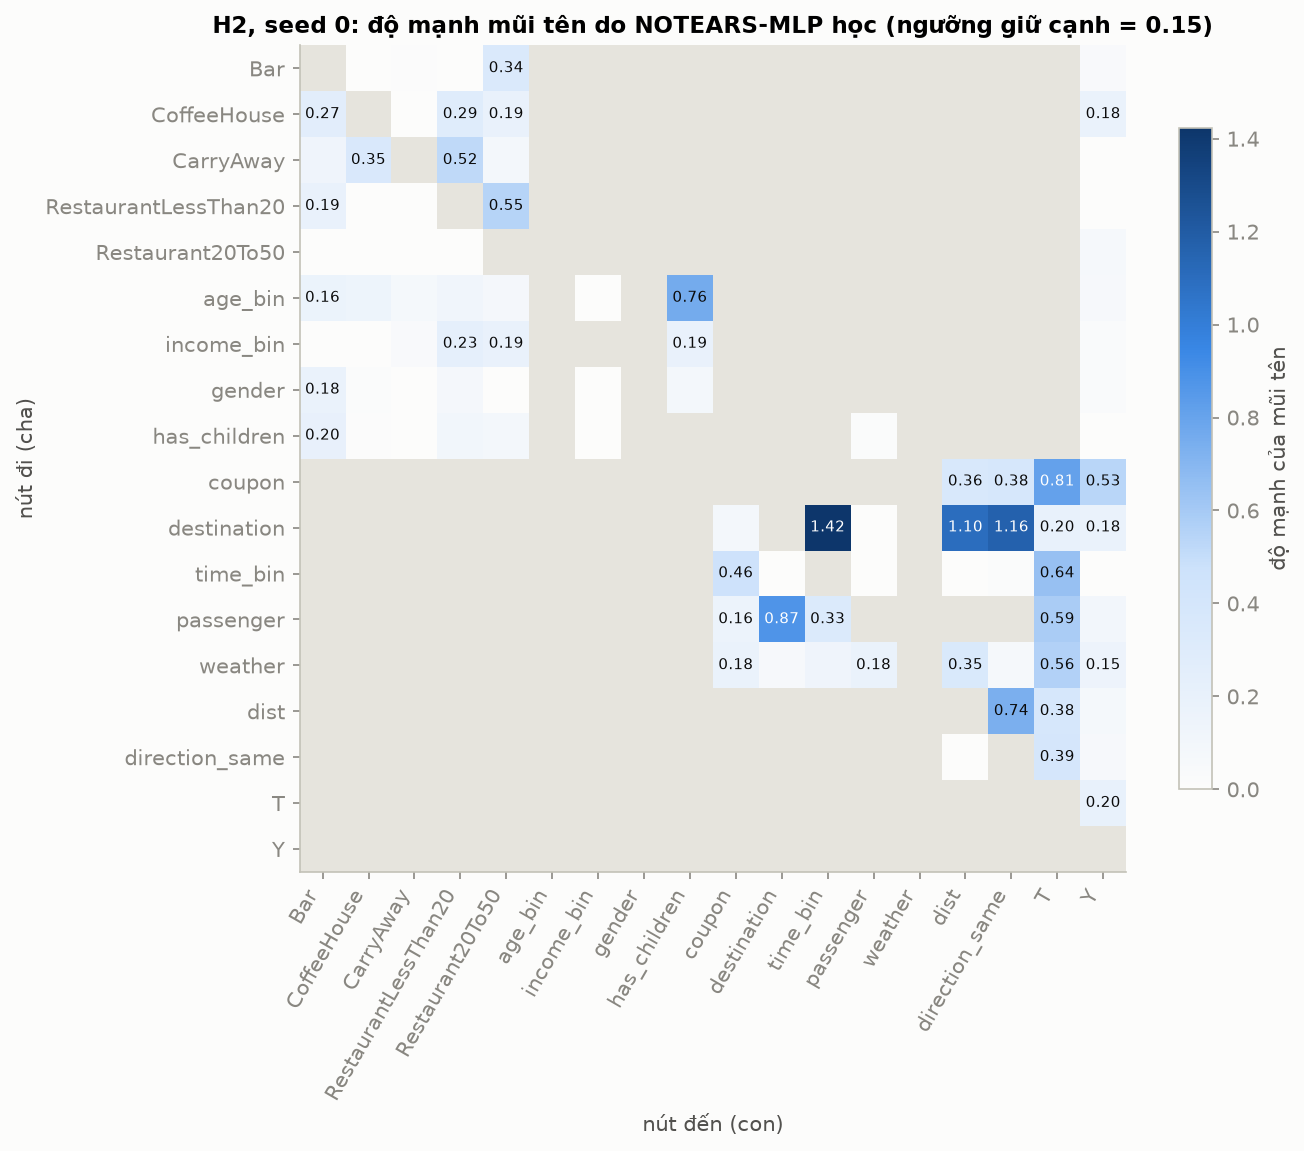
\includegraphics[width=0.92\textwidth]{figures/h2_adjacency_seed0.png}
\caption{Ma trận độ mạnh cạnh do NOTEARS-MLP học ở seed 0 (hàng: nút đi; cột: nút đến; ngưỡng giữ cạnh 0,15).}\label{fig:adj}
\end{figure}

\section{Kết quả nhận diện của DoWhy ở seed 0}\label{app:ident}

Văn bản nhận diện đầy đủ của từng DAG được lưu trong các file \texttt{identification\_b0\_seed*.txt} và \texttt{identification\_h2\_seed*.txt}. Ở seed 0, DoWhy trả về estimand loại \texttt{NONPARAMETRIC\_ATE}, viết dưới dạng $\frac{d}{d[T]}E[Y \mid Z]$, với các kết quả sau:

\begin{itemize}
\item \textbf{DAG của B0.} Backdoor: đạo hàm theo $T$ của $E[Y \mid Z]$ với $Z$ = \{\var{coupon}, \var{direction\_same}, \var{has\_children}, \var{destination}\}. Biến công cụ (iv): không tìm thấy. Frontdoor: không tìm thấy. General adjustment: $Z$ = \{\var{coupon}, \var{passenger}, \var{dist}, \var{time\_bin}, \var{weather}, \var{destination}\}.
\item \textbf{DAG của H2.} Backdoor và general adjustment: $Z$ = \{\var{coupon}, \var{weather}, \var{destination}\}. Biến công cụ: không tìm thấy. Frontdoor: không tìm thấy.
\end{itemize}

Giả định đi kèm mỗi estimand là unconfoundedness: nếu $U \to T$ và $U \to Y$ thì $P(Y \mid T, Z, U) = P(Y \mid T, Z)$ với $Z$ là tập điều chỉnh tương ứng.

\end{appendices}

\bibliography{references}

\end{document}
